\documentclass[fontsize=12pt, paper=a4, headinclude, twoside=false, parskip=half+, pagesize=auto, numbers=noenddot, open=right, toc=listof, toc=bibliography]{scrreprt}

%\usepackage[inner=4cm,outer=2cm]{geometry}
%\setlength{\oddsidemargin}{15,5pt}
%\setlength{\evensidemargin}{15,5pt}


%parskip:
  % full - Absätze haben großen Abstand
  % half - Absätze haben kleinen Abstand
  % off - Absätze haben Einzug (default)

% Bessere Unterstützung für PDF-Features
\usepackage[breaklinks=true]{hyperref}

%Schönere Schriftart laden
%\usepackage[latin1]{inputenc}
\usepackage[T1]{fontenc} % Ligaturen, richtige Umlaute im PDF
\usepackage[utf8]{inputenc}% UTF8-Kodierung für Umlaute usw
\usepackage[english]{babel} % Deutsche Silbentrennung verwenden
\usepackage{lmodern}
\renewcommand*\familydefault{\sfdefault}  %Zusatz für serifenlose Schrift.

%Zeilenabstand
\usepackage{setspace} % Zeilenabstand
\onehalfspacing % 1,5 Zeilen

% Schriften-Größen
\setkomafont{chapter}{\Huge\rmfamily} % Überschrift der Ebene
\setkomafont{section}{\Large\rmfamily}
\setkomafont{subsection}{\large\rmfamily}
\setkomafont{subsubsection}{\large\rmfamily}
\setkomafont{chapterentry}{\large\rmfamily} % Überschrift der Ebene in Inhaltsverzeichnis
\setkomafont{descriptionlabel}{\bfseries\rmfamily} % für description Umgebungen
\setkomafont{captionlabel}{\small\bfseries}
\setkomafont{caption}{\small}



% Einfachere Verwendung von korrekten Anführungszeichen
\usepackage[german=guillemets]{csquotes}
% oder german=quotes
% oder english=british oder english=american

%Mathematisches
\usepackage{amssymb}
\usepackage{amsmath}
\usepackage{amsthm}

%Quelltext einbinden
\usepackage{algorithm}
\usepackage{algorithmic}

%Abbildungen
\usepackage{graphicx}
\usepackage{caption}
\usepackage{subcaption}
\usepackage[verbose]{wrapfig}
\usepackage{float}
%\restylefloat{figure} %kannst du einen weiteren Positionierungsparameter [H] definieren. der setzt dir das bild an genau die stelle, wo du es haben willst. Ist allerdings auch nicht immer so praktisch.
% wenn du ein \pagebreak einfügst, gibt er dir vor der neuen seite noch alle gleitobjekte aus, die noch anstehen

%Zeichnen mit Tikz
\usepackage{tikz}
\usetikzlibrary{intersections,positioning,shapes.geometric,calc}

% Tabellen
\usepackage{multirow} % Tabellen-Zellen über mehrere Zeilen
\usepackage{multicol} % mehre Spalten auf eine Seite
\usepackage{tabularx} % Für Tabellen mit vorgegeben Größen
\usepackage{longtable} % Tabellen über mehrere Seiten
\usepackage{array}

%Bibliographie
\usepackage[square, comma, numbers, sort&compress, round]{natbib}
\usepackage{bibgerm} % Umlaute in BibTeX

%Umbenennung der vordefinierten definition- und example-Umgebung
\theoremstyle{definition}
\newtheorem{lecture}{Lecture}
\newtheorem{definition}{Definition}
\newtheorem{example}{Example}
\newtheorem{lemma}{Lemma}

% \newtheorem{theorem}{Satz}
% \newtheorem{constructing instructions}{Konstruktionsvorschrift}
% \newtheorem{properties}{Eigenschaften}
%\newtheorem{proposition}{Proposition}
%\newtheorem{korollar}{Corollary}
%\newtheorem{remark}{Remark}
%\newtheorem{consequences}{Consequences}
%\newtheorem{observation}{Observation}
%\newtheorem{conjecture}{Conjecture}
%\newtheorem{recall}{Recall}

\renewcommand{\labelenumi}{\roman{enumi})}

\renewcommand{\labelitemii}{$\bullet$}

\newcommand{\todo}[1]{
      {\colorbox{red}{ TODO: #1 }}
}
\newcommand{\todotext}[1]{
      {\color{red} TODO: #1} \normalfont
}

%bzgl `tocbasic` Warnung
\usepackage{scrhack}
 % Importiere die Einstellungen aus der Präambel
% hier beginnt der eigentliche Inhalt

\author{Lydia Buntrock}
\title{master thesis}
\date{Januar 2018}

\hfuzz=\maxdimen \tolerance=10000 \hbadness=10000
% \usepackage[showframe=true]{geometry}


\begin{document}
  % Titelseite
  \begin{titlepage}
    \pagestyle{empty}
  	
    	\vspace{20mm}
    	\begin{Large}
          \textbf{An analysis of maximum parsimony algorithms to predict parasitism in Eukaryota}\\
          using a large multiurcated phylogenetic synthesis tree
      \end{Large}

  	\clearpage
  \end{titlepage}

%---------------------------------------------------------------------------------------------------
%---------------------------------------------------------------------------------------------------
%---------------------------------------------------------------------------------------------------
%--------------------------------------------------------------------------------------------------- 
\chapter*{Abstract}
  This study focuses on the ancestral state reconstruction of parasitism in the tree of life of
    Eukaryota. We predict unknown states of species and estimate origins and losses of parasitism. \\
  The challenge here is the size of the tree and the little information about it. \\
  Such a large phylogenetic tree does not completely exist and therefore we work with a synthesis 
    tree of OTL \cite{Hinchliff2015} which is highly multifurcated. \\
  For the 2,535,437 leaf nodes we could not gather much data. From the GloBI database 
    \cite{Poelen2014} which we used, we could only collect 25,992 parasitic and 34,879 
    free-living species. It follows that we have only $\approx 2.4~\%$ state information. \\
  So far, especially small scale studies have been carried out or highly manual. In this scale, it 
    requires different data sources to be interconnected. \\
  We performed an analysis of existing algorithms and selected a Sankoff maximum parsimony algorithm 
    using the R package \textit{Castor} \cite{Louca2017}. \\
  Nevertheless, the results are convincing and even though purely computational approach which did 
    not include human experts input, results coincide with prior knowledge. Also regarding the number 
    of events, our estimates coincide with previous results by human experts, e.g. the study by 
    Weinstein and Kuris \cite{Weinstein2016}. \\

  ------------ \\

  \anmerkungstext{Klassisch packt man keine Referenzen in Abstracts (bzw. wenn das meist als 
    Kurzreferenz also (Author et al., 2017). (Bernhard)} \\
  We have compared the results of some subtrees with known knowledge (Chordata, Nematoda, 
    Platyhelminthes and Apicomplexa) and, except for the Nematoda, the results looked very good. In 
    the case of Nematoda, the data situation is strongly shifted to the few parasites. \\
  We could partly compare our number of origins with the results of Sara B. Weinstein and Armand M. 
  Kuris from their article \textit{Independent origins of parasitism in Animalia}  
    and have come to a similar magnitude. They identified 223 parasitic origins in Metazoa and we 
    were able to estimate about 300 origins. \\

\tableofcontents
\clearpage

%---------------------------------------------------------------------------------------------------
%---------------------------------------------------------------------------------------------------
%---------------------------------------------------------------------------------------------------
%--------------------------------------------------------------------------------------------------- 
\chapter{Introduction}
  This paper is about the analysis of ancestral state reconstruction algorithms for non-binary trees, 
    applied to the currently largest phylogeny synthesis tree of Open Tree Of Life, with the 
    application of prediciton of parasitism. \\

  \anmerkung{Mein Vorschlag einer Gliederung (jeweils ca. ein Absatz) (Bernhard)}
  \begin{enumerate}
    \item Motivation:
      \begin{itemize}
        \item Was ist das große Ziel? \\
          Das Ziel dieser Arbeit ist die Anwendung von maximum parsiomony algorithmen auf nicht 
          binäre Bäume und auf sehr große Datensätze. Insbesondere auf das Beispiel 'Entstehung des 
          Parasitismus' im ganzen Eukaryotischen Tree of Life.
        \item Was soll erreicht werden? \\
          Wir wollen vorhandene Algorithm (Sankoff/castor \cite{Louca2017}) auf diese Aufgabenstellung hin testen 
          und ihre Vorhersagekraft abschätzen. Außerdem wollen wir den Fitch algorithmus für binäre 
          Bäume auf unser Problem erweitern und mit dem Sankoff Algorithmus vergleichen.
        \item Warum ist das relevant? Was könnte man dann tun?\\
          predict states of species... \\
          \todo{!!!}
      \end{itemize}
    \item Hintergrund:
      \begin{itemize}
        \item Was gab es in dieser Richtung bereits als ganze Ansätze oder wenn nicht, warum nicht?
          Woran ist es bisher gescheitert? \\
          Bisher wurden vorallem Algorithmen für das binäre Problem entwickelt, da man wesentlich 
            kleinere Teilbäume betrachtet hat, von welchen man auch alle Aufspaltungen kennt. Durch 
            die Entwicklung von OTL, eines gesamten Baum des Lebens, ergibt sich das Problem, dass 
            dieser bei weitem nicht binär ist. \\ \\
  Researchers of the phylogenies have been dealt with the ancenstral state reconstruction in the 
    60s. The first methods were only brute force \todo{Quelle, siehe Fitch: Camin and Sokal 1965}. 
    Next came a set of parsimony algorithms such as: Fitch-parsimony \cite{Fitch1971}, 
    Wagner-parsimony \cite{Swofford1987} ... \todo{weitere?}. \\
    With more and more data, there is now the possibility to use more information to calculate the 
    probabilities of the ancestral states. In addition to the states of the leafs, algorithms could 
    also use branch lengths. The likelihood based algorithms came more in interest. \\
    Our focus came with another 'data extension'. We wanted to work with the biggest phylogenetic tree 
    that exists at this moment, which goes over all observed species. For most \todo{most?} species 
    there is no phylogeny, but only a taxonomic classification.
  
        \item Welche Grundlagen sind notwendig:
          \begin{itemize}
            \item open tree of life: Was ist das, warum relevant und überlegen als reine Ansätze? \\
              \todo{!!!} \\ \\
  So the biggest 'phylogenetic tree' is a synthesis 
    of phylogenetic trees filled with a taxonomic tree given by Open Tree of Life \cite{Hinchliff2015}.
    This tree is not binary and therefore the developed algorithms are not directly applicable. \\
            \item Algorithmen: Was gibt es? Ruhig ausführlicher als hier bereits und vor allem auch 
              nach einer Darstellung am Ende ableiten, was für uns relevant ist. Also beschreiben, 
              wie Methode a, b, c funktionieren und dann abwägen, was daher für Dich am 
              relevantesten ist. \\
              \todo{!!!} \\
              \anmerkung{GloBI und OTL in der Einleitung vorstellen. (Emanuel)}
          \end{itemize}
      \end{itemize}
    \item Outlook/Structure of this work
  \end{enumerate}


  In this work, we have looked at the algorithms that are generally suited to our data, to develop 
  them further for the not binary case, and finally to compare their usability with our sythesis 
  tree. \\
  We have decided to consider only parsimony algorithms since we have no information on branch 
  lengths and no other additional information like different transition probabilities of our states.

  In den Bacteria und Archaea wurde das mal allgemein für binary traits gemacht:
  "A total 90~\% of all binary traits described molecular functions, specifically the presence or absence of a gene or a set of gene involved in biochemical pathways."
  \cite{Goberna2015} \\
  Unterschied bei uns ist parasitismus komplexer.. da sind meist nicht einzelne Gene zuständig..

  %---------------------------------------------------------------------------------------------------
  %---------------------------------------------------------------------------------------------------
  %--------------------------------------------------------------------------------------------------- 
  \section{Definitions}
    \begin{itemize}
      \item Parasit - Freilebend
      \item Multifurkation - binär
      \item height (min, max, mean), depth of a tree/node (Distanz zur Wurzel vs distanz zum Blatt)
      \item maximum parsimony
      \item OTL, OTT, GloBI
    \end{itemize}

    Parasite \\
    Since we use Globi to classify species as parasitic or free-living, we use their definition of 
      parasitism. In GloBi, ontobee definitions are used.
    The interaction has parasite is defined as: "An interaction relationship between two organisms 
      living together in more or less intimate association in a relationship in which association is 
      disadvantageous or destructive to one of the organisms." \cite{...}. This definition includes: ecto,-
    and endoparasites, parasitoids, kleptoparasites and pathogenes.

    \todotext{Mungall, C., (2017). Definition for the interaction-term: "parasitised by; has parasite" ob
    ontobee.org. Last checked: 24.07.2017 at 
    \hyperlink{ontobee.org/ontology/RO?iri=http://purl.obolibrary.org/obo/RO_0002445}
    {ontobee.org/ontology/...}}

    Multifurcation \\
    binary or bifurcating... \cite{Felsenstein2003}

%---------------------------------------------------------------------------------------------------
%---------------------------------------------------------------------------------------------------
%---------------------------------------------------------------------------------------------------
%--------------------------------------------------------------------------------------------------- 
\chapter{Methods}
  As initiated, we would like to apply a maximum parsimony algorithm to the entire tree of life to 
    obtain an ancestral state reconstruction of free-living versus parasite states. \\
  So far, these reconstructions have been made mainly on binary trees with better data availability. 
    Therefore, we decided to use a simulation to decide how to evaluate the existing algorithms and 
    possibly adapt them to our given problem. \\
  Accordingly, in addition to the necessary data sets (GloBI, OTL), the chosen algorithm and the 
    evaluation of its results, this chapter also deals with the previously performed simulation and 
    the evaluation of the various algorithms and their parameters. \\
  Figure \ref{fig:workflow} briefly outlines these relationships.
  \begin{figure}[h!]
    \centering
    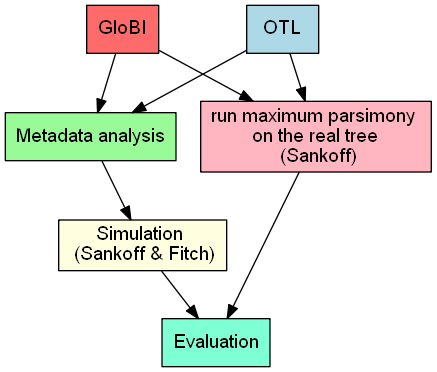
\includegraphics[width=0.55\textwidth]{Figures/Workflow-overview.png}
    \caption{Workflow \\
      The coming sections are thus subdivided into the following topics: \\
      \todo{or:} The resulting procedure is as follows: \\
      (1) Get the real tree and real data for the leaf nodes $\rightarrow$ OTL, GloBI databases.
      (2) Get metadata of these for a realisitc the simulation.
      (3) Build and run the simulation.
      (4) Evaluation of parameters for the simulation and the real problem.
      (5) Run the resulted algorithm on the original data.
      (6) Evalute and interprete results. $\rightarrow$ Origins etc...
    }
    \label{fig:workflow}
  \end{figure}

  % \begin{enumerate}
  %   \item Get the real tree and real data for the leaf nodes. $\rightarrow$ OTL, GloBI databases
  %   \item Get metadata of these for a realisitc the simulation.
  %   \item Build and run the simulation.
  %   \item Evaluation of parameters for the simulation and the real problem.
  %   \item Run the resulted algorithm on the original data.
  %   \item Evalute and interprete results. $\rightarrow$ Origins etc...
  % \end{enumerate}
  
  \begin{figure}[h!]
    \centering
    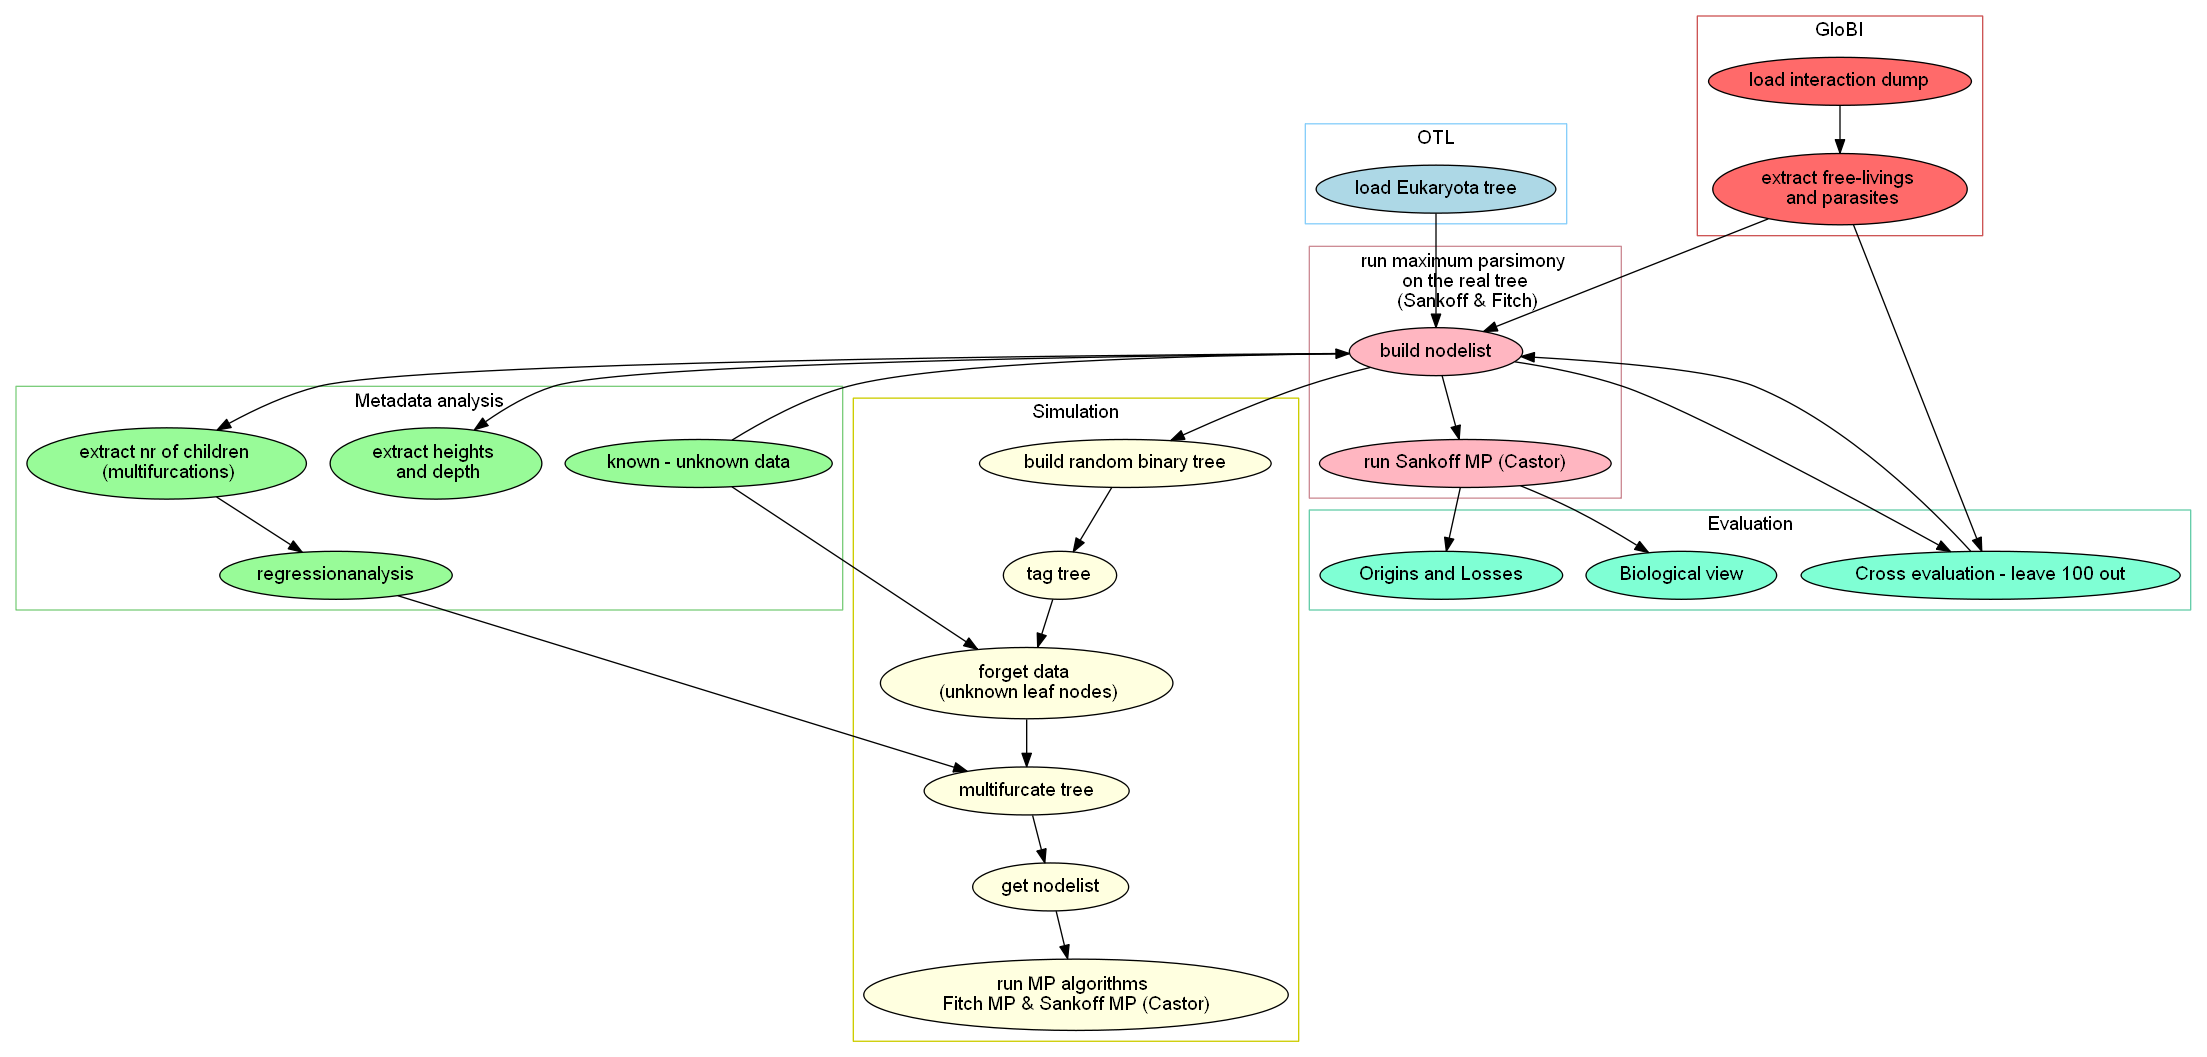
\includegraphics[width=1\textwidth]{Figures/Workflow.png}
    \caption{Big overview of the whole Workflow}
    \label{fig:Workflow}
  \end{figure}

  %---------------------------------------------------------------------------------------------------
  %---------------------------------------------------------------------------------------------------
  %---------------------------------------------------------------------------------------------------
  \section{Get data - Properties of real Data}
    For our research we need two types of data: a tree and information about the states. \\
    For the tree we decided to use Open Tree of Life (OTL). \\
    For the state information, we decided to use the Global biotic interaction database (GloBI).

    %---------------------------------------------------------------------------------------------------
    %---------------------------------------------------------------------------------------------------
    \subsection{OTL}
      For our project we looked for a large database for phylogenetic trees and also for a taxonomic 
        tree. Since we run our algorithm on the phylogenetic tree, and for the evaluation and other 
        properties the taxonomy provides us with much more information. \\
      OTL gives us both. A synthesis of phylogenetic trees (currently 819 trees) and a taxonomic tree. 
        OTL also includes the large phylogenetic database TreeBASE \cite{Hinchliff2015}. \\
      \todo{Das steht auf der Website nicht in dem Paper...} \\
      For phylogenetic data, there are at least five big data collections, namely: ITIS (Integrated 
        Taxonomic Information System) \cite{ITIS}, NCBI (National Center for Biotechnology Information) 
        \cite{NCBI1988}, WORMS (World Register of Marine Species) \cite{WoRMS2018}, GBIF (Global 
        Biodiversity Information Facility) \cite{GBIF}, OTT (OpenTreeOfLife-Taxonomy) 
        \cite{Hinchliff2015}. \\
      \todotext{Marius:} "Every dataset has it's own characteristics and downsides. ITIS is only a small 
        set of 100~\% confirmed and named species. GBIF is not composed with the help of phylogeny, the 
        same is valid for the NCBI taxonomy. The WORMS taxonomy is a way too small dataset of mostly 
        marine species. \\
      We choosed the taxonomy from OpenTreeOfLife because it's including most of the known taxonomies 
        and got synthesised by preffering taxonomies that match with available phylogenetic data. At the 
        same time the team from OTL preferred a maximum number of species \cite{Hinchliff2015}. This is 
        resulting in somekind of hybrid between taxonomy and phylogeny." \\

      We took a closer look at some of the features of the Synthesis tree. On the one hand the 
        distribution of the taxa and on the other the distribution of the nodes on the taxa. Since this
        is not directly relevant to our study, there is a section in the appendix \ref{sec:otl analysis}.

    %---------------------------------------------------------------------------------------------------
    %---------------------------------------------------------------------------------------------------
    \subsection{GloBI}
      \todotext{Marius:} "There aren't many big active interaction databases out there, most of them are 
        offline or outdated. For example: IWDB (Interaction Web Database) \cite{IWDB2003}, Webs on the 
        Web \cite{WOW2004}, Animal Diversity Web \cite{Myers2003} and ecoweb \cite{Cohen2010}. GloBI is 
        including most of the known ones and is still growing actively \cite{Poelen2014}. So the 
        question which interaction database could be used was answered rather quickly." \\

      This database consists of entries of the form: species A (source) interacts with B (target). \\
      We appointed some interactions\footnote{\hyperlink{
        https://github.com/jhpoelen/eol-globi-data/blob/master/eol-globi-lib/src/main/java/org/eol/globi/domain/InteractType.java
        }{https://github.com/jhpoelen/eol-globi-data/.../InteractType.java}}
        , where we know from the biological perspective that the species source or target has to be a 
        parasite or a free-living species. These are the following:
      \begin{itemize}
        \item free-living source: preysOn, eats, flowersVisitedBy, hasPathogen, pollinatedBy, 
          hasParasite, hostOf
        \item free-living target: preyedUponBy, parasiteOf, visitsFlowersOf, pathogenOf, hasHost
        \item parasite source: parasiteOf, pathogenOf
        \item parasite target: hasParasite, hasPathogen
      \end{itemize}
      We build two lists: parasites and free-livings, and add the source or targets of an interaction
        to these.

  %---------------------------------------------------------------------------------------------------
  %---------------------------------------------------------------------------------------------------
  %---------------------------------------------------------------------------------------------------
  \section{Metadata analysis}
    In order to generate the most realistic simulation, influencing parameters were investigated. \\
    There are two major types of parameters:
    \begin{enumerate}
      \item Biological parameters (A result of the evolutionary process.):
        \begin{itemize}
          \item transition probabilities
        \end{itemize}
      \item Distribution of the loss of information:
        \begin{itemize}
          \item Loss of topology ($\rightarrow$ mutlifurcations)
          \item Unknown information about states of some leaf nodes
        \end{itemize}
    \end{enumerate}
    We tested the influence of these parameters on our result using our simulation (Section 
      \ref{sec:simulation}).
   
    %---------------------------------------------------------------------------------------------------
    %---------------------------------------------------------------------------------------------------
    \subsection{Transition probabilities}
      This subsection deals with the transition probabilities from free-living (hereinafter / as a 
        formula FL) to parasitic (hereinafter P) and vice versa: $\mathcal{P}(FL \rightarrow P)$, 
        $\mathcal{P}(P \rightarrow FL)$. \\
      Different parasite types have different transition probabilities. It is very difficult to make a 
        statement about these probabilities.
      In general, we assume that there are 40~\% parasites and 60~\% free-livings which is based on the 
        estimates by Windsor \cite{Windsor1998} and 
        $\mathcal{P}(FL \rightarrow P) > \mathcal{P}(P \rightarrow FL)$, because a reverse mutation is 
        usually less likely. \todo{This is discussed in section x of the discussion.} \\

      For the maximum parsimony analysis of the real data, all transition probabilities were equated.
        However, the used castor package \cite{Louca2017} offers the possibility to enter different 
        transition probabilities.
      \begin{wrapfigure}{r}{0.5\textwidth}
        \begin{center}
          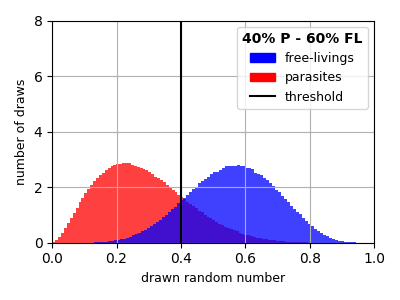
\includegraphics[trim = 0mm 0mm 0mm 15mm, clip, width=0.48\textwidth]{Figures/40-60.png}
        \end{center}
        \caption{60~\% Free-living - 40~\% Parasites \\ red: parasites, blue: free-living, \\ the threshold is at 0.4}
        \label{fig:Beta distribution}
      \end{wrapfigure}

      In the simulation, we chose two beta distributions and a threshold that indicates the change 
        between states. \\
      Different thresholds with different beta distributions were simulated, with different distributions 
        of parasites and free-livings: 50~\% P to 50~\% FL, 40~\% P to 60~\% FL, 30~\% P to 70~\% FL and 
        20~\% P to 80~\% FL (\todo{see results simulation, ref...}). Figure \ref{fig:Beta distribution} 
        shows one example of these. \\
      \todo{Plot neu erstellen: Achsenbeschriftung, threshold}

    %---------------------------------------------------------------------------------------------------
    %---------------------------------------------------------------------------------------------------
    \subsection{Missing information}

      A binary tree with $n$ leaf nodes has $n-1$ internal nodes. The present Eukaryota tree of OTL has 
        2,293,463 leaf nodes and only 41,974 internal nodes, that is:
      $$100-\frac{100}{(2293463-1) \times 41974} \approx 98.16 \%$$
        missing internal nodes. \\

      % \anmerkungstext{Nested models were compared using likelihood ratio tests, models using different 
      %   predictors were compared according to their deviance and AIC. (Emanuel)} \\

      For the present Eukaryota tree with 2,293,463 leaf nodes, 34,869 free-livings and 25,962 parasites 
        are found, which are
        $$100-\frac{100}{2293463 \times (34860+25962)} \approx 97.34 \%$$
        unknown states of leaf nodes. \\

      In the simulation, the influence of the multifurcations and missing data in leaf nodes on the 
        predictive accuracy of the ancestral state reconstruction algorithms is tested. \\
      For the real data, generalized linear models are compared with poisson respectively binomial 
        regression according to their residuals and BICs.

  %---------------------------------------------------------------------------------------------------
  %---------------------------------------------------------------------------------------------------
  %---------------------------------------------------------------------------------------------------
  \section{Simulation}\label{sec:simulation}
    There are various possibilities of ancestral state reconstruction. The simulation compared 
      different algorithms. \\
    On the one hand different implementations of the Fitch maximum parsimony were compared and on the 
      other hand the best of them with the implementation of the sankoff algorithm of the castor 
      package \cite{Louca2017}. \\

    \begin{figure}[h!]
      \centering
      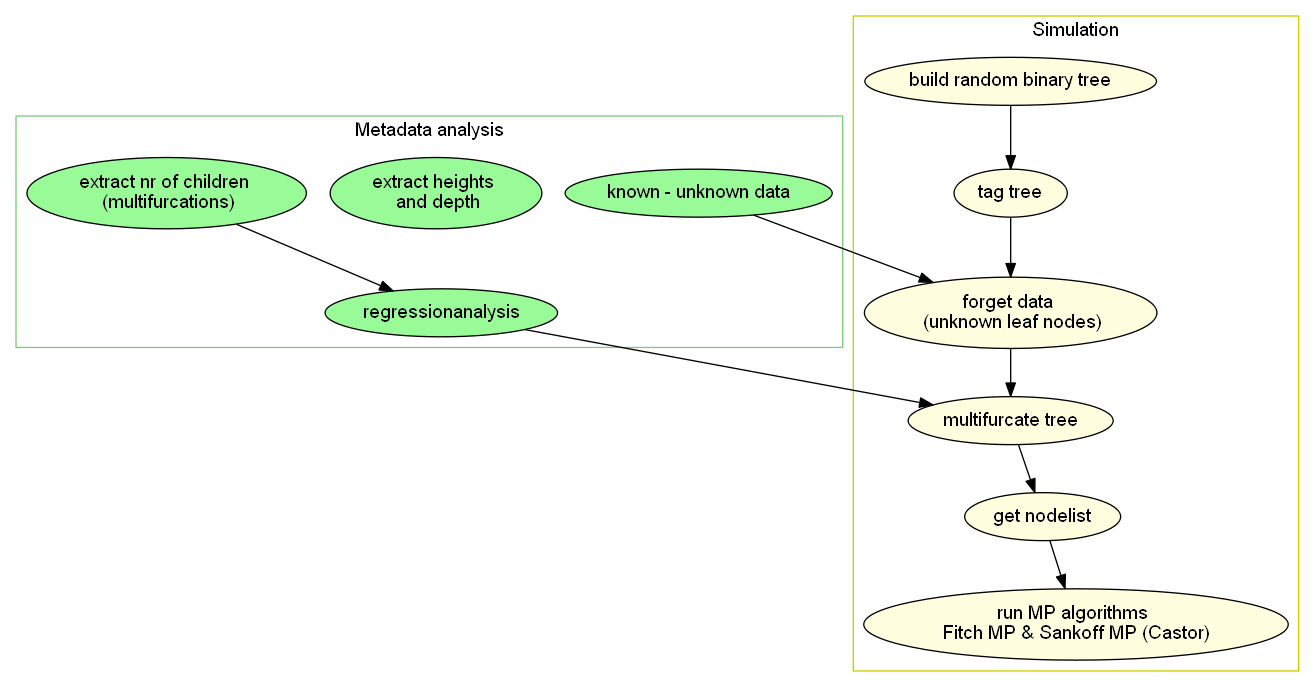
\includegraphics[width=1\textwidth]{Figures/Workflow-Simulation.png}
      \caption{Course of the simulation with influence of the metadata analysis from the real data.}
      \label{fig:Simulation Workflow}
    \end{figure}

    Figure \ref{fig:Simulation Workflow} shows the course of the simulation. The individual steps are 
      explained in the following subsections.

    \todo{Evaluation - compare trees (distances)}

    %---------------------------------------------------------------------------------------------------
    %---------------------------------------------------------------------------------------------------
    \subsection{random binary tree}
      You need a tree to do a simulation of ancestral state reconstruction. It had to be decided whether 
        to take the real tree or simulate a tree. In this simulation, trees were created randomly, as 
        one can replicate a complete binary phylogentic tree. Thus, there is also the possibility to 
        simulate the multifurcation. \\
      
      To get a random binary tree, the Phylo package from biopython were used \cite{Cock2009}. They offer 
        a randomized function which returns a BaseTree\footnote{
          \hyperlink{https://github.com/biopython/biopython/blob/master/Bio/Phylo/BaseTree.py}
          {https://github.com/biopython/biopython/blob/master/Bio/Phylo/BaseTree.py}
        }. \\
      \todo{ref in die discussion über die randomized function? Diskutieren wir das?}

    %---------------------------------------------------------------------------------------------------
    %---------------------------------------------------------------------------------------------------
    \subsection{simulating states and transitions between them}
      The next step is to simulate the states of the nodes using the transitions. Again, we simulate 
        fully known states and then 'forget' everything but a few in the leaf nodes so that you can 
        later compare the reconstruction with the origin. \\
      The root node (ancestor of all subsequent species) is (of course) free-living. That means it will 
        start in the free-living beta distribution. Now traverse from the root to the leaf nodes, always 
        pulling out of the current distribution until you get above the threshold and the new node 
        changes state. \\
      To ensure that the parameter of the binomial distribution is restricted to the [0,1] interval, we 
        model it with a beta distribution as in Figure \ref{fig:Beta distribution}. \\

      After traversing through the tree, each state is saved in a nodelist associated with the node ID 
        which is the OTT from OTL. \\

% simulate loss of information
      Here begins the simulation of the lost information. This is on the one hand the states and on the 
        other the topology of the tree. Some splits of nodes are unknown with which the tree is 
        multifurcated (explained in the following section \todo{pageref}). \\

      In the real tree, there is usually only information about species living today $\rightarrow$ leaf 
        nodes. And beyond only a small percentage of these. All information about the states of the 
        internal node and one leaf node is 'forgotten' and stored in another column to the node. \\
      Different percentages of forgetting the information were simulated, as you can read in the 
      \todo{section ... from the results}.

    %---------------------------------------------------------------------------------------------------
    %---------------------------------------------------------------------------------------------------
    \subsection{simulating loss of information of the tree topology}
      As previously explained, some divisions in the tree are not known, so the real tree is not binary.
      This multifurcation was simulated by an equally distributed percentage of forgotten internal nodes.

    %---------------------------------------------------------------------------------------------------
    %---------------------------------------------------------------------------------------------------
    %---------------------------------------------------------------------------------------------------
    \section{Ancestral state reconstruction methods}
      For about 50 years, people have been working on ancestral state reconstruction. The first paper 
        mentioned above is by Camin and Sokal, who in 1965 were working on algorithms for discrete-state 
        data \cite{Camin1965}. Different methods have been developed and the question is which method is 
        the most suitable for our problem. \\
      For this purpose, various studied methods and their advantages and disadvantages were compared. \\
    
      Royer-Carenzi et al. distinguishes two major classes of ancestral state reconstruction methods: \\
      The first is to explain the current state with the least number of state changes between an 
        ancestor and his child, this is called parsimonious. \\
      The other class she presents involves modeling the character evolution as a stochastic process and 
        using the likelihoods to compute the possible ancestral character states. This is generally done 
        with a continuous time Markov model \cite{RoyerCarenzi2013}. \\

      \todo{Pasqualin et al. unterscheiden noch eine weitere Methode: stochastic mapping...} \\

      One of the major disadvantages of parsimony methods is that, unlike likelihood approaches, they 
        can not take divergece times (branch length) into account. Since we have no development times in 
        our case, you can ignore this. \\
      Another problem pointed out by Royer-Carenzi is that parsimony approaches are either based on 
        predefined parameters (generalized parsimony) or on strong and often controversial assumptions, 
        like irreversibility for dollo parsimony. Again, this problem is irrelevant for us, because you 
        can only work with generalized models in the analysis of the entire Eukaryota tree. \\

      Following the principle of the simpler model first, the decision has \todo{fallen?} on parsimonious 
        methods since these are sufficient for the case present here. \\
      Felsenstein \cite{Felsenstein2003} discusses in his book two algorithms that generalize all 
        previous methods (from Camin and Sokal \cite{Camin1965}, \todo{Kluge and Farris} and Farris 
        \cite{Farris1970}): Fitch parsiomony \cite{Fitch1971} and Sankoff parsimony \cite{Sankoff1975}. \\
      \anmerkungstext{Unter Farris war auch noch der Begriff Wagner trees in gebrauch, als 
        Verallgemeinerung der parsimonious trees von Camin und Sokal. (Lydia)} \\
      \todo{Wagner-parsimony \cite{Swofford1987}} \\
      
      Thus, the methods used in this work are those of Fitch and Sankoff. For Fitch, the algorithm has 
        been extended from binary to multifurcated trees. For the Sankoff algorithm, Louca and Doebeli 
        have presented an implementation for non-binary trees published in an R package named 
        \textit{castor} \cite{Louca2017}.

      %---------------------------------------------------------------------------------------------------
      %---------------------------------------------------------------------------------------------------
      \subsection{Fitch maximum parsimony}
        Fitch maximum parsimony is an algorithm for rooted, binary trees and describes an ancestral state 
          reconstruction for discrete states \cite{Fitch1971} by minimizing transitions between states. \\
        Note, the original Fitch algorithm has the sole purpose of minimizing the number of transitions 
          and not reconstructing the ancestral nodes. Felsenstein \cite{Felsenstein2003} describes a 
          simple extension for the reconstruction. Cunningham et al. \cite{Cunningham1998} have refined 
          these. \todotext{Wir haben mit ein paar kleinen änderungen optimiert... und schließlich auf 
          multifurcated angepasst...} \todotext{eigentlich ist Cunningham 'nur' eine kritische 
          Neubewertung. Sie beziehen ihren Algortihmus auf Swofford und Maddison...} \\
        To understand the differences to the multifurcated case, the algorithm for the binary case is 
          briefly explained and referred to the extension. \\
          \begin{wrapfigure}[19]{r}{0.5\textwidth}
            \centering
            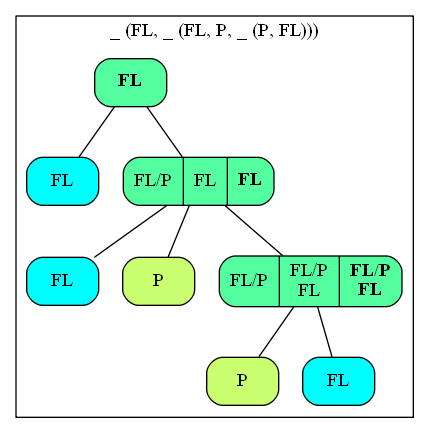
\includegraphics[width=0.4\textwidth]{Figures/Fitch1.png}
            \caption{Fitch algorithm for binary trees. \\
              The unknown leaf node is discribed with both states. Computed internal nodes (exclusive the 
              root node) consists of three sets, where the last set is the final one (bold). \\
              From the second internal node (seen from the root node) there are several possibilities to 
              create the second and third set.}
            \label{fig: binary Fitch}
          \end{wrapfigure}
        Input: A rooted, binary tree, with state informations in the leaf nodes. Each node is depicted as 
          a set of states. There are only two states in this paper, free-living (FL) and parasitic (P). 
          Internal nodes have three sets, which are empty at the beginning, excluding the root node, it 
          has only one. Leaf nodes have their state as a set (eg \{FL\} or \{P\}, unknown leaf nodes the 
          union of all possible states (\{FL, P\}). \\
        The algorithm traverses three times trough the tree and fills these sets. \\
        In each step, two sets are considered and their intersect formed. There are two cases:
        \begin{enumerate}
          \item The intersection is not empty and corresponds to the new set.
          \item The intersection is empty. $\rightarrow$ Build the union of these sets as new set.
        \end{enumerate}
        First traverse from the leaf nodes to the root / move down the tree / postorder tree traversal. 
          Each internal node is formed from its child nodes, where at the beginning the only information
          lies. \\
        Second traverse from the root node to the leafs. Each internal node is formed from its father node 
          and its sibling node. \\
        Last traversion (direction does not matter): Build the final state for every node. It is formed 
          from the sets of previous traversals. \\
        (The original Fitch algorithm was designed to minimize transitions without predicting actual states 
          of internal nodes, so it was just the first traversal.) \\
        The extension to the non-binary case is quite obvious, but holds some opportunities. In this case, 
          more than two children may be present for the first traversal, but the incision or union may 
          also be formed over more than two sets. Also in the second traversing, there may be several 
          sibling nodes. However, there are several possibilities here that were all tested and compared 
          in the simulation. Some of these options are already available in the binary case:
        \begin{itemize}
          \item The father node has (except for the root node) two state sets, because he came through 
            the up-traversing previously. Are both sets used or only the first traversing?
          \item Since there are several siblings, do you first of all make the cut or union, or directly 
            in the whole with the father node?
        \end{itemize}
        The first point already has an effect on the binary case. Figure \ref{fig: binary Fitch} shows 
          both possibilities of the three sets. \\
        Cunningham uses only the first state set of the father node \cite{Cunningham1998}. \\
        From these two points four different versions of Fitch were formed:
        \begin{enumerate}
          \item Fitch 1: First state set of father node; intersection/union of siblings first.
          \item Fitch 2: First state set of father node; intersection/union of siblings together with father node.
          \item Fitch 3: Both state sets of father node; intersection/union of siblings first.
          \item Fitch 4: Both state sets of father node; intersection/union of siblings together with father node sets.
        \end{enumerate}
        \begin{figure}
          \centering
          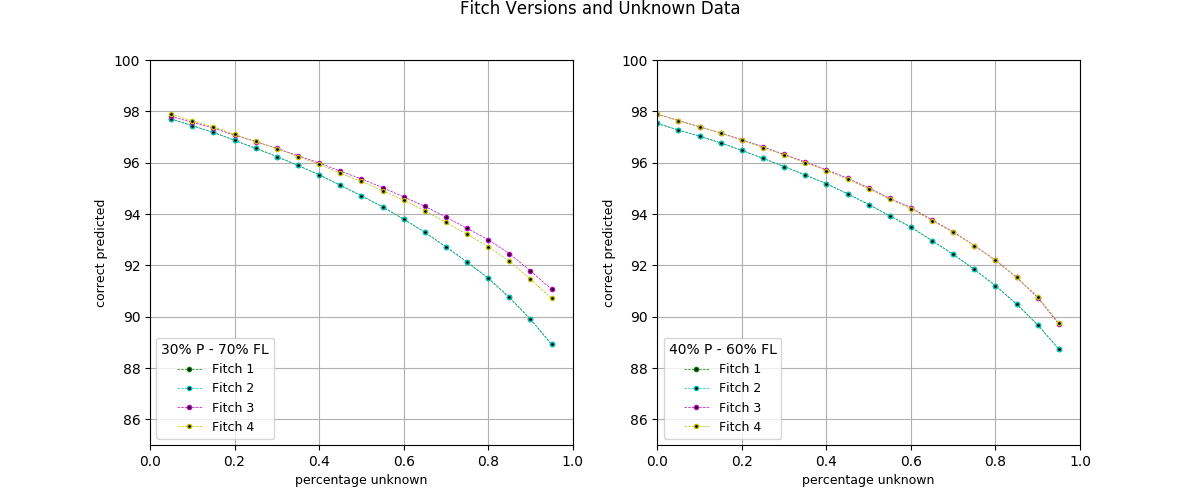
\includegraphics[width=0.8\textwidth]{Figures/simulation_fitch_evaluation.png}
          \caption{Test of Fitch Versions.}
          \label{fig:Fitch versions}
        \end{figure}
        These four versions were tested in the simulation with 100 trees and 10000 leaf nodes and a
          distribution of 60~\% FL to 40~\% P. Figure \ref{fig:Fitch versions} shows this over all unknown 
          node percentage. \\
        At 90~\% unknown nodes and 90~\% of multifurcation of the internal nodes, version 1 was 89.26~\%, 
          version 2 was 89.26~\%, version 3 was 89.35~\%, and version 4 was 89.31~\% correct. Therefore, 
          only version 3 was used for all further simulations.


      %---------------------------------------------------------------------------------------------------
      \subsubsection{Sankoff}
        Maximum parsimony algorithm from Sankoff implemented in the R package castor \cite{Louca2017}. \\
        \todo{transition probabilities: all equal}

  % %---------------------------------------------------------------------------------------------------
  % %---------------------------------------------------------------------------------------------------
  % %---------------------------------------------------------------------------------------------------
  % \section{real data analysis}
  %   \begin{itemize}
  %     \item Import tree
  %     \item Import interactions
  %     \item run castor algorithm / and others?
  %     \item interprete results (cross validation - leave 100 out)
  %   \end{itemize}

  %---------------------------------------------------------------------------------------------------
  %---------------------------------------------------------------------------------------------------
  %---------------------------------------------------------------------------------------------------
  \section{Implementation}
    You can find the full code on GitHub: 
      \hyperlink{github.com/Irallia/IZW-HU-Parasites}{github.com/Irallia/IZW-HU-Parasites}. \\
    Most of the code was written in Python. The analyzes and the use of the Castor package in R. There 
      are some shell scripts to execute whole workflows.

%---------------------------------------------------------------------------------------------------
%---------------------------------------------------------------------------------------------------
%---------------------------------------------------------------------------------------------------
%---------------------------------------------------------------------------------------------------
\chapter{Results}
  A big point in this chapter is the result of examining the input data. How is the situation? What 
    influence does that have on our actual result? What can we do about it? Our simulation gave us 
    some results to this. \\
  Otherwise, this chapter is mainly about the actual reconstruction of the states. This means, on 
    one hand investigation of origins and losses of the inner nodes and on the other, the prediction 
    of unknown states of leaf nodes. \\
   
  %---------------------------------------------------------------------------------------------------
  %---------------------------------------------------------------------------------------------------
  %---------------------------------------------------------------------------------------------------
  \section{Metadata analysis}
    %---------------------------------------------------------------------------------------------------
    %---------------------------------------------------------------------------------------------------
    \subsection{Missing information}
      As previously presented, we have two types of missing information: unknown states of leaf nodes 
        and multifurcation. \\

      We examined the ridge of multifurcation of the tree. A complete phylogenetic tree would be 
        binary, which means the number of leaf nodes is closely to the number of internal nodes. But 
        since we only work with a synthesis tree, this tree is multifurcated: we have 241 974 internal 
        nodes and 2 293 463 leaf nodes. \\
      \begin{figure}[h]
        \centering
        \begin{subfigure}[b]{0.5\textwidth}
          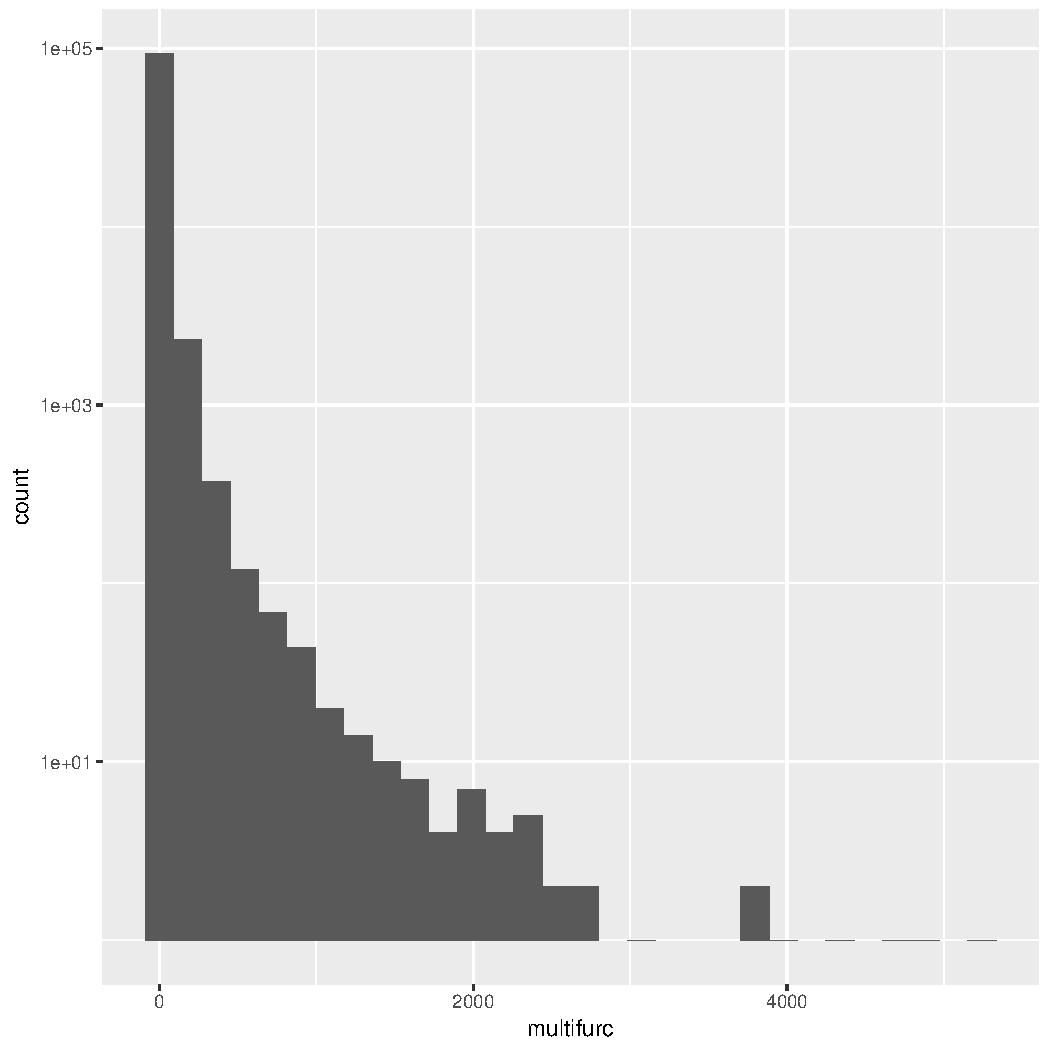
\includegraphics[width=\textwidth]{Figures/multifurc.pdf}
          \caption{Histogram with automatic binwidth. \\ ~ \\ ~}
        \end{subfigure}
        ~~~ %add desired spacing between images, e. g. ~, \quad, \qquad, \hfill etc. 
          %(or a blank line to force the subfigure onto a new line)
        \begin{subfigure}[b]{0.42\textwidth}
          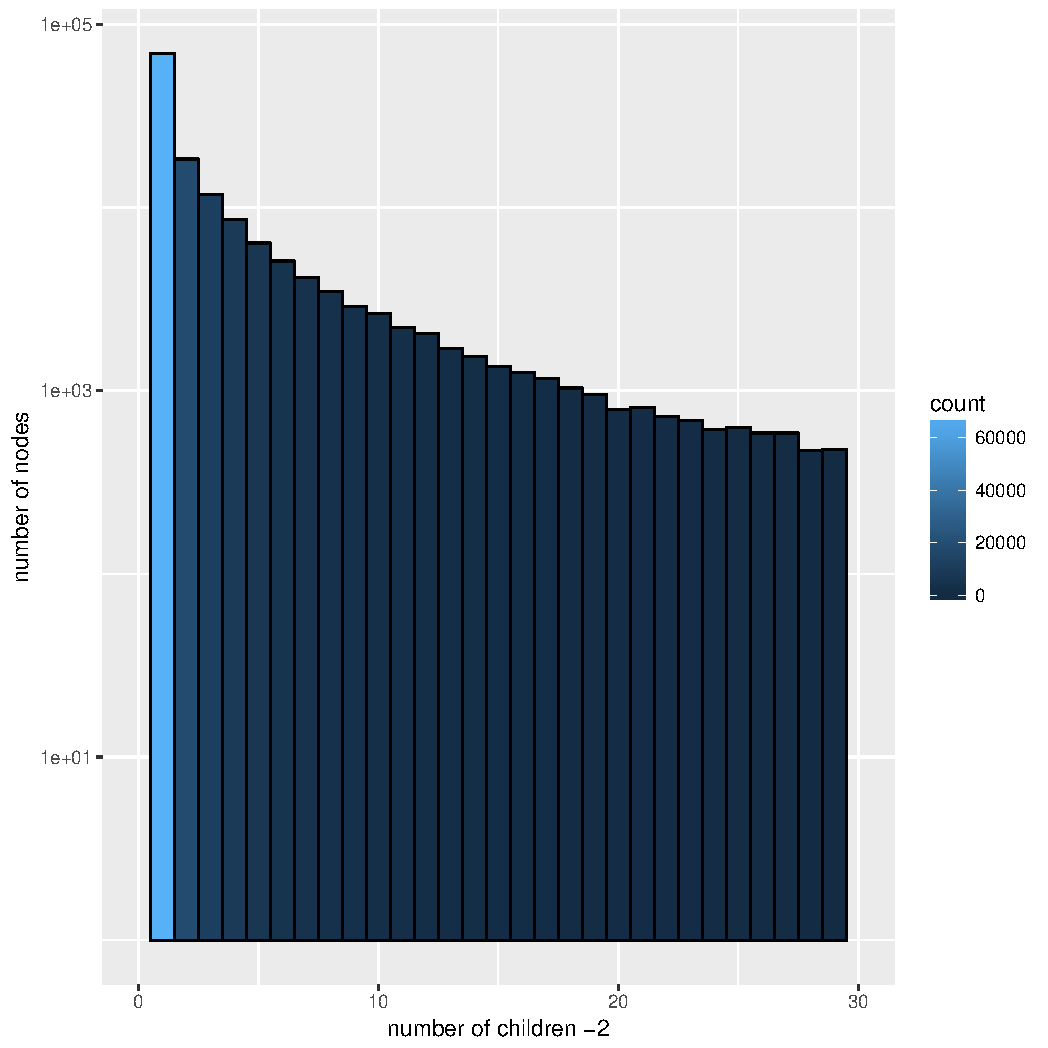
\includegraphics[trim = 0mm 0mm 30mm 0mm, clip, width=\textwidth]{Figures/multifurc_small.pdf}
          \caption{Histogram with $binwidth = 1$. \\ light blue: binary; dark blue: multifunction}
        \end{subfigure}
        \caption{Histograms about the multifurcation of the internal nodes of the synthesis tree.}
        \label{fig:childrenOfNodes}
      \end{figure}

      For a first overview we collected for every node its number of children (degree $-1$), and plotted
        this in two histograms, see figure \ref{fig:childrenOfNodes}. \\
      The multifurcation affects only the internal nodes. We collected the number of children $-2$ of 
        every node (a node with two children is binary). That means it discribes the number of nodes which we have lost from the real (binary) 
      phylogenetic tree. \\
      As you can see, we are very far from a binary tree. \\

      Some subtrees have been examined, these have the following percentages of missing information: See 
        table \ref{table:percentage loss information subtrees}.

      \begin{table} [h]
        \begin{center}
          \begin{tabular}{ |l|r|r||r|r|r| }
            \hline
            Domain  & \% unknown states & \% multifurcation \\ 
            / Kingdom  & (missing state information & (missing \\
            / Phylum / Class & of leaf nodes) & internal nodes) \\
            \hline \hline
            Eukaryota       & 97.34~\%  & 98.16~\% \\
            \hline \hline
            Metazoa         & 96.44~\%  & 87.93~\% \\ \hline
            Fungi           & 98.87~\%  & 96.97~\% \\ \hline
            Chloroplastida  & 99.14~\%  & 89.46~\% \\
            \hline \hline            
            Arthropoda      & 97.49~\%  & 89.95~\% \\ \hline
            Apicomplexa     & 86.26~\%  & 87.16~\% \\ \hline
            Nematoda        & 89.01~\%  & 88.59~\% \\ \hline
            Chordata        & 88.59~\%  & \cellcolor{green!50}66.49~\% \\ \hline
            Platyhelminthes & \cellcolor{green!50}68.73~\%  & 80.34~\% \\
            \hline \hline            
            Insecta         & 97.11~\%  & 90.78~\% \\
            \hline  
          \end{tabular}
        \end{center}
        \caption{Examination of subtrees regarding missing information}
        \label{table:percentage loss information subtrees} 
      \end{table}

      %---------------------------------------------------------------------------------------------------
      \subsubsection{Data artifacts}
        At this point we also found out that there are some nodes with only one child node (55700 nodes). \\
        These are both, the most nodes are right in front of a leaf, as well as some nodes are deep in the 
          tree (3956 with height $>2$). They are probably a result from the fact that taxonomic information 
          has been incorporated into a phylogeny. \\
        Some examples:
        \begin{itemize}
          \item Nephroselmidophyceae: (class) \\
            https://tree.opentreeoflife.org/opentree/argus/ottol@1038762
          \item Phrynocrinidae: (family) \\
            https://tree.opentreeoflife.org/opentree/argus/ottol@3647979
          \item Elaeocarpus sylvestris: \\
            https://tree.opentreeoflife.org/opentree/argus/opentree9.1@ott166969
        \end{itemize}

      %---------------------------------------------------------------------------------------------------
      \subsubsection{Taxa}
        The investigation of the taxonomy revealed that our tree has three kingdoms: Chloroplastida, 
          Metazoa, Fungi, 53 phyla, 195 classes and 924 orders. \\
        Since the analysis of the tree is not part of this work, it should be mentioned here that, 
          according to recent findings, this is not complete and we lack some taxa in every rank. For 
          example, Cavalier-Smith says that one distinguishes between seven and nine kingdoms 
          \cite{CavalierSmith1981}. \\
        In section \pageref{subsec:listPhyla} of the appendix you can find a list of all phyla.

      %---------------------------------------------------------------------------------------------------
      \subsubsection{Poisson regression of the multifurcation}
        % glm (generalized linear model) analysis: \\
        The intercept is $2.821 > 0$ $\Rightarrow$ there is a multifunction.
        (Intercept: Stärke der Multifurcation) \\
        Comparing the different kingdoms, we find that multifunctionality is greater in Fungi than in 
        Chloroplastida than in Metazoa:
        $$4.0999 (Fungi Intercept) > -0.9132 (Chloroplastida Intercept) > -1.4320 (Metazoa Intercept)$$
        % Degrees of Freedom: 96010 Total (i.e. Null);  96010 Residual
        Wir haben außerdem drei komplexitätsstärken von Modellen verglichen bezüglich der höhe und tiefe 
          des Baums mit dem folgenden Deviance Table:

        \begin{table}[h]
          \begin{center}
              \begin{tabular}{ |l|r|r|r|r|r| }
                \hline
                Model / Taxa & Kingdom & Phylum & Class & Order & Family \\
                \hline \hline
                multifurc $\sim$ taxa & 7774454 & \cellcolor{green!10}7435700 & \cellcolor{green!15}7337241 & \cellcolor{green!30}7076068 \\
                \hline
                multifurc $\sim$ taxa + depth & 7752303 & \cellcolor{green!10}7431609 & \cellcolor{green!15}7334754 & \cellcolor{green!30}7027578 \\
                multifurc $\sim$ taxa + max.height & 7730196 & \cellcolor{green!15}7375889 & \cellcolor{green!20}7275856 & \cellcolor{green!30}7005424 \\
                multifurc $\sim$ taxa + min.height & \cellcolor{green!10}7472500 & \cellcolor{green!20}7233486 & \cellcolor{green!25}7144686 & \cellcolor{green!40}6890703 \\
                multifurc $\sim$ taxa + mean.height & \cellcolor{green!15}7304402 & \cellcolor{green!25}7128318 & \cellcolor{green!30}7055313 & \cellcolor{green!40}6815271 \\
                \hline
                multifurc $\sim$ taxa * depth & 7714881 & \cellcolor{green!15}7335396 & \cellcolor{green!20}7250759 & \cellcolor{green!40}6843004 \\
                multifurc $\sim$ taxa * max.height & \cellcolor{green!5}7692980 & \cellcolor{green!15}7311241 & \cellcolor{green!25}7187504 & \cellcolor{green!45}6795823 \\
                multifurc $\sim$ taxa * min.height & \cellcolor{green!10}7442387 & \cellcolor{green!25}7177002 & \cellcolor{green!30}7094933 & \cellcolor{green!45}6795099 \\
                multifurc $\sim$ taxa * mean.height & \cellcolor{green!20}7247309 & \cellcolor{green!30}7020258 & \cellcolor{green!35}6965794 & \cellcolor{green!50}6665565 \\
                \hline
              \end{tabular}
          \end{center}
          \caption{Residuals...}
          \label{table:...} 
        \end{table}
        * Residuals: Fehler - wieviele Werte sind nicht gut modelliert. (umso kleiner umso besser - grün) \\

        Interpretation: Die Multifurkation ist sehr ungleich verteilt. Daher ist die vorhersage umso 
          genauer umso kleinere Subtrees wir betrachten. ...
        
        Because of the difference in the complexity of the models, we compared their BICs:
        \begin{table}[h]
          \begin{center}
            \begin{tabular}{ |l|r|r|r|r|r| }
              \hline
              Model / Taxa & Kingdom & Phylum & Class & Order & Family \\
              \hline \hline
              multifurc $\sim$ taxa & 8273333 & \cellcolor{green!15}7937828 & \cellcolor{green!20}7842157 & \cellcolor{green!30}7644249 \\
              multifurc $\sim$ taxa & 8257680 & \cellcolor{green!15}7922207 & \cellcolor{green!20}7826490 & \cellcolor{green!35}7574154 \\
              \hline
              multifurc $\sim$ taxa + depth & 8273318 & \cellcolor{green!15}7934322 & \cellcolor{green!20}7839364 & \cellcolor{green!35}7539999 \\
              multifurc $\sim$ taxa + max.height & \cellcolor{green!15}7993515 & \cellcolor{green!25}7749121 & \cellcolor{green!30}7661817 & \cellcolor{green!40}7416211 \\
              multifurc $\sim$ taxa + min.height & 8251211 & \cellcolor{green!20}7875521  & \cellcolor{green!25}7778327 & \cellcolor{green!35}7516883 \\
              multifurc $\sim$ taxa + mean.height & \cellcolor{green!20}7825417 & \cellcolor{green!30}7644249 & \cellcolor{green!35}7572474 & \cellcolor{green!45}7340741 \\
              \hline
              multifurc $\sim$ taxa * depth & 8235932 & \cellcolor{green!20}7836755 & \cellcolor{green!25}7757688 & \cellcolor{green!45}7383808 \\
              multifurc $\sim$ taxa * max.height & \cellcolor{green!15}7963438 & \cellcolor{green!30}7693555 & \cellcolor{green!30}7614820 & \cellcolor{green!45}7335338 \\
              multifurc $\sim$ taxa * min.height & 8214030 & \cellcolor{green!20}7808940 & \cellcolor{green!30}7690618 & \cellcolor{green!45}7336627\\
              multifurc $\sim$ taxa * mean.height & \cellcolor{green!25}7768360 & \cellcolor{green!35}7536296 & \cellcolor{green!50}7484953 & \cellcolor{green!50}7206369 \\
              \hline
            \end{tabular} 
          \end{center}
          \caption{BIC...}
          \label{table:...} 
        \end{table}

      %---------------------------------------------------------------------------------------------------
      \subsubsection{Binomial regression of the unknown state information}

        Next to the problem of the multifurcation of the tree is the less of data we have for the species.
          For the ancestral state reconstruction, we need information in the leaf nodes. \\
        The eukaryotic synthesis tree has 293 463 leaf nodes. The GloBI database has 5 346 414 interactions 
          (at this timepoint). Out of this data we got 51 337 distinct free-living species and 47 332 
          distinct parasite species $\rightarrow$ unknown nodes 2194794 ($\approx 95.7~\%$). \\
        We found also $57,352$ (not distinct) source species and $809,993$ (not distinct) target
          species without OTT ids. Since we currently use only OTT ids, we could not use this information. \\
        \todo{With this only $\approx 4.3~\%$ information in our leaf nodes are ...} \\
        We also compared different models in terms of their BICs (Table: \ref{table:BIC unknown information}). 
          The Residuals are not very meaningful here, since all models have different dimensions.

        \begin{table}[h!]
          \begin{center}
            \begin{tabular}{ |l|r|r|r| }
              \hline
              Model / Taxa & Kingdom & Phylum & Class \\
              \hline \hline
              multifurc $\sim$ taxa & 545740 & \cellcolor{green!10}499227 & \cellcolor{green!30}482265 \\
              \hline
              multifurc $\sim$ taxa + depth & 544789 & \cellcolor{green!10}493017 & \cellcolor{green!50}478998 \\
              \hline
              multifurc $\sim$ taxa * depth & 544062 & \cellcolor{green!30}488366 & \cellcolor{green!50}476382 \\
              \hline
            \end{tabular}
          \end{center}
          \caption{Residuals of unknown information}
          \label{table:...}
        \end{table}

        \begin{table}[h!]
          \begin{center}
            \begin{tabular}{ |l|r|r|r|r| }
              \hline
              Model / Taxa & Kingdom & Phylum & Class & Order \\
              \hline \hline
              multifurc $\sim$ taxa & \cellcolor{green!15}545799 & \cellcolor{green!35}500004 & \cellcolor{green!45}485121 & XXXXX \\
              \hline
              multifurc $\sim$ taxa + depth & \cellcolor{green!15}544862 & \cellcolor{green!40}493808 & \cellcolor{green!45}481869 & \cellcolor{green!50}478851 \\
              \hline
              multifurc $\sim$ taxa * depth & \cellcolor{green!15}544179 & \cellcolor{green!45}489845 & \cellcolor{green!45}481494 & \cellcolor{green!50}478188 \\
              \hline
            \end{tabular} 
          \end{center}
          \caption{BICs of unknown information}
          \label{table:BIC unknown information} 
        \end{table}

        \todo{Taxa like order or family were too expensive to calculate...}



    %---------------------------------------------------------------------------------------------------
    %---------------------------------------------------------------------------------------------------
    \subsection{Results of simulation / Influence of different parameters}

      As presented, we compare two methods in our simulation to their prediction accuracy: Fitch and 
        Sankoff. \\
      We examine different parameters. In figure \ref{fig:influence of unknown data} is an overview of 
        the results. \\
      The first column describes the distributions of free-livings and parasites with a given threshold 
        for the respective simulations to the right. \\
      The middle column investigates the influence of the unknown states, the right the influence of the 
        strength of the multifurcation. \\
      The y-axes indicate the percentage of correctly predicted states (including known states). On the 
        x-axis the percentage of forgotten states or missing internal nodes. \\
      Each point corresponds to the average of one hundred simulations, each with 10,000 leaf nodes. \\
      For the middle column we set the strength of the multifurcations to 0.95\% similar to the real 
        data and in the right column the amount of the unknowns to 0.95\% also similar to the real data. \\

      As you can see both algortithms are always over 50\% and therefore better than guessing. Moreover, 
        they are usually close to each other, with Sankoff always makes better predictions except for 
        equally distributed states as Fitch. \\
      You can see that the distribution of states has a strong influence on the prediction. The more 
        evenly distributed, the harder it is to predict. \\
      If more than 60\% of internal nodes are missing, Fitch breaks significantly in his prediction 
        compared to Sankoff.
      
      \begin{figure}
        \centering
        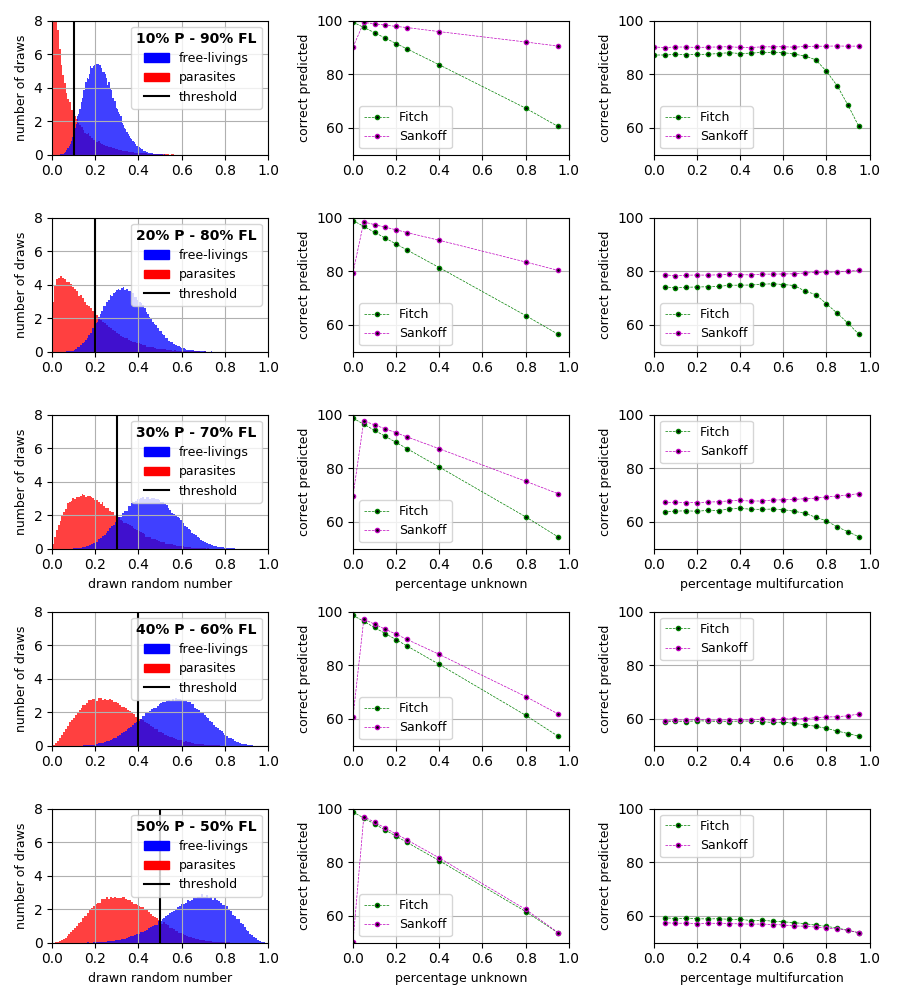
\includegraphics[trim = 0mm 0mm 0mm 0mm, clip,width=\textwidth]{Figures/simulation_evaluation_1.png}
        \caption{Influence of unknown data to prediction}
        \label{fig:influence of unknown data}
      \end{figure}

      In the end, Sankoff is in most cases the more accurate algortihmus and was therefore used for our 
        prediction of the real data.

  %---------------------------------------------------------------------------------------------------
  %---------------------------------------------------------------------------------------------------
  %---------------------------------------------------------------------------------------------------
  \section{Results of castor}

    %---------------------------------------------------------------------------------------------------
    %---------------------------------------------------------------------------------------------------
    \subsection{Biological view}

      \todo{Castor replaces originaltags with finaltags. There are 82 originaltags != finaltag.} \\

      We picked a few phyla to evaluate the results from the biological point of view. \\
      Table \ref{table:phylum leaf nodes states} shows some known phyla: Chordata, Nematoda, 
        Platyhelminthes and Apicomplexa. \\
      Since GloBI is not perfect, all examples contain a few bugs.

      \todo{\ref{table:table:percentage loss information subtrees}} \\


      As known the Chordata are full of free-living species and there are only a few parasites. Among 
        the birds are some breeding parasites (brood parasitism) like the cuckoo and clepto-parasites as 
        the skuas \cite{Rothschild1957}. The algorithm reflects this. We started with 99.83~\% 
        free-living species and predicted 99.94~\% species as parasites \todo{(inklusive all known nodes)}. 
        Only 0.06~\% were predicted as parasites. \\
      \todo{We found the cuckoo and some skuas...?} \\
      Same observation but with less free-livings is the Apicomplexa Phylum. Here we have only a few 
        free-livings \todo{ref einfügen}. And as we see, we had good start data and predicted 00.95~\% as 
        parasites. \\
      For the Platyhelminthes the literature says that there are mostly all Platyhelminthes parasites
        \todo{ref einfügen}. But at the end we predicted 4.18~\% as free-living. The class Seriata is the 
        reason for the most of free-livings in this phylum. These are partly free-living flatworms, so 
        the prediction looks right. \\
        \todotext{ Wiki: \\
        *The Seriata are an order of turbellarian flatworms.[1][2] \\
        They are found in both freshwater and marine environments, and also include a number of species 
        found in damp terrestrial conditions. Most are free-living, but the group includes the genus 
        Bdelloura, which lives comensally on the gills of horseshoe crabs. Seriatans are distinguished 
        from other related groups by the presence of a folded pharynx and of a number of diverticula 
        arising from the intestine. The intestine itself may be either simple or branched.[3]}
      
      With the Nematoda it looks very different. In the Nematoda its much worse. Most Nematoda are 
        free-living, but we found only 2.63~\% of them. Blaxter et al. speaks of at least seven 
        independently arosed parasitism \cite{Blaxter1998}. In a recent article Blaxter identifies 18 
        origins \cite{Blaxter2015} in Nematoda. \\
        The problem at this point, however, is obvious: The parasites have been much more studied and 
        thus we start with only 0.63~\% free-living species. Against such a shifted data situation, the 
        algorithm is almost powerless. And yet the percentage has increased.

        The evolution of parasitism in Nematoda: \\
        "while only approximately 23 000 species have been described (J. Hallan, unpublished; https://insects.tamu.edu/research/collection/hallan/), the true species-level diversity may be 1 million or more (Lambshead, 1993)." \\
        " Estimates of the number of species of parasitic nematode per host suggest that there may be of the order of 25 000 nematode parasites just of vertebrates, most of which remain undescribed (Dobson et al. 2008)" \\
        "a large proportion of nematode species may be parasites." \cite{Blaxter2015} \\

      \begin{table}
        \begin{center}
          \hspace*{-1cm}\begin{tabular}{ |l|r||r|r||r|r|r|r|r|r| }
            \hline
            & & \multicolumn{2}{c||}{original states} & \multicolumn{6}{c|}{final states} \\
            Phylum & \# nodes & FL & P
              & 0 (FL) & 0.4 & 0.5 & 0.67 & 0.75 & 1 (P) \\
            \hline \hline
            Chordata & 91785 & 10451 & 18 
              & 91734 & 0 & 0 & 0 & 0 & 51 \\
            & & 99.83~\% & 0.49~\%
              & 99.94~\% & & & & & 0.06~\% \\ \hline
            Nematoda & 30127 & 21 & 3289 
              & 791 & 0 & 1017 & 0 & 0 & 28319 \\
            & & 0.63~\% & 99.37~\%
              & 2.63~\% & & 3.38~\% & & & 94~\% \\ \hline
            Platyhelminthes & 22683 & 7 & 7086 
              & 949 & 0 & 151 & 0 & 0 & 21583 \\
            & & 0.1~\% & 99.9~\%
              & 4.18~\% & & 0.67~\% & & & 95.15~\% \\ \hline
            Apicomplexa & 1863 & 1 & 255 
              & 1 & 0 & 0 & 0 & 0 & 1862 \\
            & & 0.39~\% & 99.61~\%
              & 0.05~\% & & & & & 99.95~\% \\
            \hline \hline
            Arthropoda & 1198981 & 18912 & 11141 
              & 1099509 & 1313 & 22478 & 4176 & 1665 & 70223 \\
            & & 62.93~\% & 37.07~\%
              & 91.7~\% & 0.11~\% & 1.87~\% & 0.35~\% & 0.14~\% & 5.86~\% \\
            \hline
          \end{tabular} 
        \end{center}
        \caption{Phylum (leaf nodes)}
        \label{table:phylum leaf nodes states} 
      \end{table}

      \anmerkungstext{Das sind schonmal vier große Kontraste, wenn dann noch Zeit bleibt, die 
        schwirigen... Arthropoden, Fungi, Pflanzen... (Emanuel)} \\

      \begin{table}
        \begin{center}
          \hspace*{-2cm}\begin{tabular}{ |l|r||r|r||r|r|r|r|r|r|r|r| }
            \hline
            & & \multicolumn{2}{c||}{original states} & \multicolumn{8}{c|}{final states} \\
            Kingdom & \# nodes & FL & P
              & 0 (FL) & 0.25 & 0.33 & 0.4 & 0.5 & 0.67 & 0.75 & 1 (P) \\
            \hline \hline
            none & 84456 & 45 & 529 
              & 15035 & 243 & 25910 & 0 & 8764 & 6183 & 0 & 28140 \\
            Fungi & 324105 & 577 & 2983
              & 39088 & 0 & 0 & 0 & 5858 & 0 & 0 & 274803 \\
            Chloroplastida & 460457 & 3519 & 77
              & 454211 & 0 & 0 & 0 & 4688 & 0 & 0 & 1558 \\
            Metazoa & 1670956 & 30758 & 22373
              & 1485749 & 0 & 0 & 1313 & 29002 & 5102 & 1957 & 147833 \\
            \hline  
          \end{tabular}
        \end{center}
        \caption{Kingdom (inkl internal nodes)}
      \end{table}

      \begin{table}
        \begin{center}
          \begin{tabular}{ |l|r||r|r||r|r|r|r|r|r| }
            \hline
            & & \multicolumn{2}{c||}{original states} & \multicolumn{6}{c|}{final states} \\
            Phylum & \# nodes & FL & P
              & 0 (FL) & 0.4 & 0.5 & 0.67 & 0.75 & 1 (P) \\
            \hline \hline
            Chordata & 122546 & 10451 & 18 
              & 122473 & 0 & 0 & 0 & 0 & 73 \\
            Nematoda & 33564 & 21 & 3289 
              & 846 & 0 & 1133 & 0 & 0 & 31585 \\
            Platyhelminthes & 27142 & 7 & 7086 
              & 1010 & 0 & 175 & 0 & 0 & 25957 \\
            Apicomplexa & 2102 & 1 & 255 
              & 1 & 0 & 0 & 0 & 0 & 2101 \\
            \hline
            Arthropoda & 1319460 & 18912 & 11141 
              & 1207204 & 1313 & 25499 & 4852 & 1957 & 78635 \\
            \hline
          \end{tabular}
        \end{center}
        \caption{Phylum (inkl internal nodes)}
      \end{table}

      \begin{table}
        \begin{center}
          \hspace*{-2cm}\begin{tabular}{ |l|r||r|r||r|r|r|r|r|r|r|r| }
            \hline
            & & \multicolumn{2}{c||}{original states} & \multicolumn{8}{c|}{final states} \\
            Kingdom & \# nodes & FL & P
              & 0 (FL) & 0.25 & 0.33 & 0.4 & 0.5 & 0.67 & 0.75 & 1 (P) \\
            \hline \hline
            none & 75446 & 45 & 529 
              & 13426 & 220 & 24082 & 0 & 7792 & 5302 & 0 & 24493 \\
            Fungi & 31457 & 577 & 2983
              & 38520 & 0 & 0 & 0 & 5723 & 0 & 0 & 266463 \\
            Chloroplastida & 416478 & 3519 & 77
              & 410795 & 0 & 0 & 0 & 4182 & 0 & 0 & 1501 \\
            Metazoa & 1491012 & 30758 & 22373
              & 1328135 & 0 & 0 & 930 & 25535 & 4423 & 1665 & 130324 \\
            \hline  
          \end{tabular}
        \end{center}
        \caption{Kingdom (leaf nodes)}
      \end{table}

    %---------------------------------------------------------------------------------------------------
    %---------------------------------------------------------------------------------------------------
    \subsection{Origins and Losses}

      Weinstein and Kuris have been searching for origins of parasitism in Animalia \cite{Weinstein2016}. 
        They identified 223 parasitic origins: 223 in Metazoa $\supset$ 143 in Arthropoda $\supset$ 87 
        in Insecta. \\
      This has led us to count the origins and losses of parasitism in our investigation as well. \\
      We count only one origin / loss in a parent node with different children's nodes. \\
      Here we have encountered a problem: The Castor algorithm gives us probabilities for states. That 
        means there are also nodes with state like 0.3 or 0.5. So how do you count? Our solution was, 
        to round these values. We have to say that we round 0.5 to 0.

      \begin{table} [h]
        \begin{center}
          \begin{tabular}{ |l|r|r||r|r|r| }
            \hline
            Domain  & \# internal & \# leaf & Rootnode & \multicolumn{2}{c|}{without and with rounding} \\ 
            / Kingdom  & \multicolumn{2}{c||}{nodes} & state & \# origins & \# losses \\
            / Phylum / Class & & & & (FL -> P) & (P -> FL) \\
            \hline \hline
            Eukaryota & 241974 & 2293463 & 1.0 & 415 & 363 \\
            & & & P & 462 & 369 \\
            \hline \hline
            Metazoa & 179944 & 1491012 & 0.5 & 294 & 123 \\
            & & & & 321 & 129 \\ \hline
            Fungi & 9534 & 314571 & 0.5 & 80 & 222 \\
            & & & & 97 & 222 \\ \hline
            Chloroplastida & 43486 & 412434 & 0.0 & 40 & 2 \\
            & & & FL & 42 & 2 \\
            \hline \hline            
            Arthropoda & 120479 & 1198981 & 0.0 & 260 & 102 \\
            & & & FL & 281 & 108 \\ \hline
            Apicomplexa & 239 & 1863 & 1.0 & 0 & 1 \\
            & & & P & 0 & 1 \\ \hline
            Nematoda & 3437 & 30127 & 1.0 & 0 & 11 \\
            & & & P & 2 & 11 \\ \hline
            Chordata & 30761 & 91785 & 0.0 & 12 & 1 \\
            & & & FL & 12 & 1 \\ \hline
            Platyhelminthes & 4459 & 22683 & 1.0 & 0 & 5 \\
            & & & P & 0 & 5 \\
            \hline \hline            
            Insecta & 91256 & 989572 & 0.0 & 234 & 77 \\
            & & & FL & 245 & 77 \\ 
            \hline  
          \end{tabular}
        \end{center}
        \caption{Origins and losses}
        \label{table:origins and losses} 
      \end{table}

      In Table \ref{table:origins and losses} we can see, that we found some more origins than Weinstein 
        and on top of that some losses. \\
      
      Lets have a look at the same phyla as in the section before: Chordata, Nematoda, 
        Platyhelminthes and Apicomplexa. \\
      Chordata are full of free-living species and so we see only a few origins of parasitism. The root
      and mostly all species are predicted as free-living. \\
      In Apicomplexa and the Platyhelminthes are looking fine too. Our algorithm gives us only one loss 
        of parasitism in Apicomplexa and five in the Platyhelminthes. They are both from the root over 
        mostly all species predicted as parasites. \\
      Nematoda is again full of problems. The rootnode is predicted as a parasite and so we have more 
        losses of parasitism for the less information of free-living species in this phylum. The rest 
        is parasitic \\
        As we have already mentioned Blaxter et al. found at least seven origins of parasitism 
          \cite{Blaxter1998}. If we assume that the root node of Nematoda is free-living, then some 
          losses would have to turn around and become Origins. So it could be that we end up in a similar 
          size as Blaxter.

      \begin{lstlisting}[gobble=6]
        # possible tags: 0, 0.333, 0.4, 0.5, 0.667, 0.75, 1
        # rounded to:    0  0      0    0    1      1     1
        if node_state != father_state:
          if father_state == 0:
              origins += 1        # FL -> P
              new_found = True
          else:
              losses += 1         # P -> FL
              new_found = True
      \end{lstlisting}

      \todo{without rounding change else: to elif $father_state == 1$}
      
    %---------------------------------------------------------------------------------------------------
    %---------------------------------------------------------------------------------------------------
    \subsection{Cross evaluation - leave 100 out}
      We ran the castor algorithm 100 times with leaving 100 randomized free-living or parasitic species 
        out of the input data to see how stable our result is. Of these 10,000 nodes, 9,238 were unique. 
        Of that, we predicted 9060 ($\approx 98.17~\%$) correctly and 169 ($\approx 1.82~\%$) wrongly, with 
        duplicate draws always having the same prediction. \\
      What is the best way to model this data? We again tested the influence of the taxa and the depth of 
        leaf nodes and calculated the BICs (Table: \ref{table:BIC cross validation}).

      \begin{table}[h]
        \begin{center}
          \begin{tabular}{ |l|r|r|r|r| }
            \hline
            Model / Taxa & Kingdom & Phylum & Class & Order \\
            \hline \hline
            correct predicted $\sim$ taxa & XXXXX & XXXXX & XXXXX & XXXXX \\
            \hline
            correct predicted $\sim$ taxa + depth & 117703 & XXXXX & XXXXX & XXXXX \\
            \hline
            correct predicted $\sim$ taxa * depth & 117592 & XXXXX & XXXXX & \cellcolor{green!60}XXXXX \\
            \hline
          \end{tabular} 
        \end{center}
        \caption{Residuals of cross validation prediction}
        \label{table:Residuals cross validation} 
      \end{table}

      \begin{table}[h]
        \begin{center}
          \begin{tabular}{ |l|r|r|r|r| }
            \hline
            Model / Taxa & Kingdom & Phylum & Class & Order \\
            \hline \hline
            correct predicted $\sim$ taxa & 117936 & 112242 & XXXXX & XXXXX \\
            \hline
            correct predicted $\sim$ taxa + depth & 117776 & XXXXX & XXXXX & XXXXX \\
            \hline
            correct predicted $\sim$ taxa * depth & XXXXX & XXXXX & XXXXX & \cellcolor{green!60}XXXXX \\
            \hline
          \end{tabular} 
        \end{center}
        \caption{BICs of cross validation prediction}
        \label{table:BIC cross validation} 
      \end{table}

      Resiudals:
      \begin{itemize}
        \item correct predicted $\sim$ 1: 120325
        \item correct predicted $\sim$ kingdom: 117877
        \item correct predicted $\sim$ phylum: 111466
      \end{itemize}

      What could happen by removing a parasite or free-living of the list?
      \begin{itemize}
        \item It could be a specie, which don't exist in the tree leaf nodes. -> no effect
        \item It could be a specie, which exists in both lists. -> If it was a parasite, it is now 
          free-living, because we prefer parasites. Otherwise we have no effect again. (1053 are possible)
        \item Normal case: We loose information, because its a specie in our tree and we change it to a 
          leave node with no information.
      \end{itemize}

      Influence on the rest of the data:
      \begin{table}
        \begin{center}
          \begin{tabular}{ |cl||r|r|r|r|r| }
            \hline
            & & min & max & mean & variance ($\sigma^2$) & $\sigma$ \\
            \hline \hline
            \multirow{3}{*}{distance} & all   & 0 & 3587.70 & 224.96 & 313650.61 & 560.05 \\
            & leaf nodes                      & 0 & 3021.12 & 208.69 & 248103.38 & 498.10 \\
            & internal nodes                  & 0 & 566.58 & 16.28 & 4927.95 & 70.20 \\ \hline
            \multicolumn{2}{|c||}{changed tag} & 0 & 0 & 0 & 0 & 0 \\ \hline
            \multirow{3}{*}{lost} & all tags  & 100 & 100 & 100 & 0 & 0 \\
            & FL tags                         & 44 & 66 & 57.25 & 19.50 & 4.42 \\
            & P tags                          & 34 & 56 & 42.75 & 19.50 & 4.42 \\
            \hline
          \end{tabular}
        \end{center}
        \caption{Statistics to Cross validation}
      \end{table}

      \begin{table}
        \begin{center}
          \begin{tabular}{ |cl||r|r|r|r| }
            \hline
            & & min & max & mean & variance \\
            \hline \hline
            \rowcolor{green!50}distance & all   & 1 & 2 & 1.33 & 0.33 \\
            \rowcolor{orange!50}&               & 0 & 3587.70 & 217.94 & 273760.68 \\
            \rowcolor{green!50}& leaf nodes     & 1 & 2 & 1.33 & 0.33 \\
            \rowcolor{orange!50}&               & 0 & 3021.12 & 202.57 & 209274.86 \\
            \rowcolor{green!50}& internal nodes& 0 & 0 & 0.00 & 0.00 \\
            \rowcolor{orange!50}&               & 0 & 566.58 & 15.37 & 5684.00 \\ \hline
            \rowcolor{green!50}lost & FL tags   & 44 & 49 & 46.67 & 6.33 \\
            \rowcolor{orange!50}&               & 51 & 66 & 57.95 & 13.47 \\
            \rowcolor{green!50}& P tags         & 51 & 56 & 53.33 & 6.33 \\
            \rowcolor{orange!50}&               & 34 & 49 & 42.05 & 13.47 \\
            \hline
          \end{tabular}
        \end{center}
        \caption{Statistics to Cross validation \\
          - \colorbox{green!50}{Less free-livings - 3 examples} \\
          - \colorbox{orange!50}{Less parasites - 64 examples}}
      \end{table}

  %---------------------------------------------------------------------------------------------------
  %---------------------------------------------------------------------------------------------------
  %---------------------------------------------------------------------------------------------------
  \section{Effects of Taxa in the different models}

    The comparisons of the effects of the taxa can be found in Table \ref{table:Effects unknown data} 
    and showed ...

    \begin{table}[h!]
      \begin{center}
        \begin{tabular}{ |l|l|r|r|r|r| }
          \hline
          Taxa & Model / Effects & min & max & mean & median \\
          \hline \hline
          Kingdom & globi $\sim$ taxa         & 0,01 & 0,04 & 0,02 & 0,01 \\
                  & globi $\sim$ taxa + depth & 0,01 & 0,03 & 0,02 & 0,01 \\
                  & globi $\sim$ taxa * depth & 0,00 & 0,03 & 0,01 & 0,01 \\
          \hline
          Phylum & globi $\sim$ taxa          & 0,17 & 393501,80 & 32208,79 & 6149,78 \\
                  & globi $\sim$ taxa + depth & 0,32 & 567010,90 & 55149,54 & 10783,18 \\
                  & globi $\sim$ taxa * depth & 0,00 & 1000000,00 & 225375,33 & 2511,58 \\
          \hline
        \end{tabular} 
      \end{center}
      \caption{Effects of Taxa in models for unknown data}
      \label{table:Effects unknown data} 
    \end{table}

    globi $\sim$ taxa * depth: NOTE: kingdom is not a high-order term in the model

    \begin{figure}[h!]
      \centering
      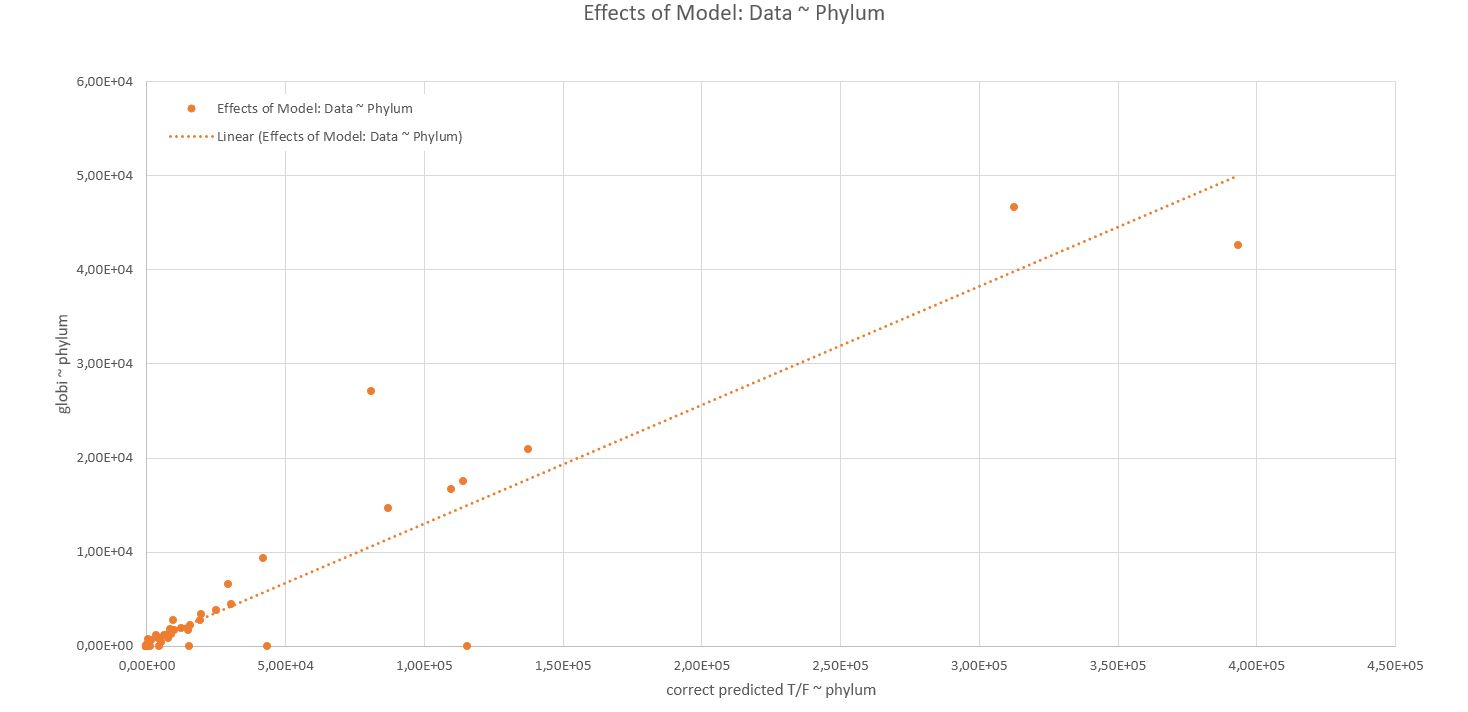
\includegraphics[trim = 0mm 0mm 0mm 15mm, clip, width=\textwidth]{Figures/EffectsOfModel-Data-Phylum.JPG}
      \caption{Effects of Model: Data $\sim$ Phylum}
      \label{fig:...}
    \end{figure}
    \begin{figure}[h!]
      \centering
      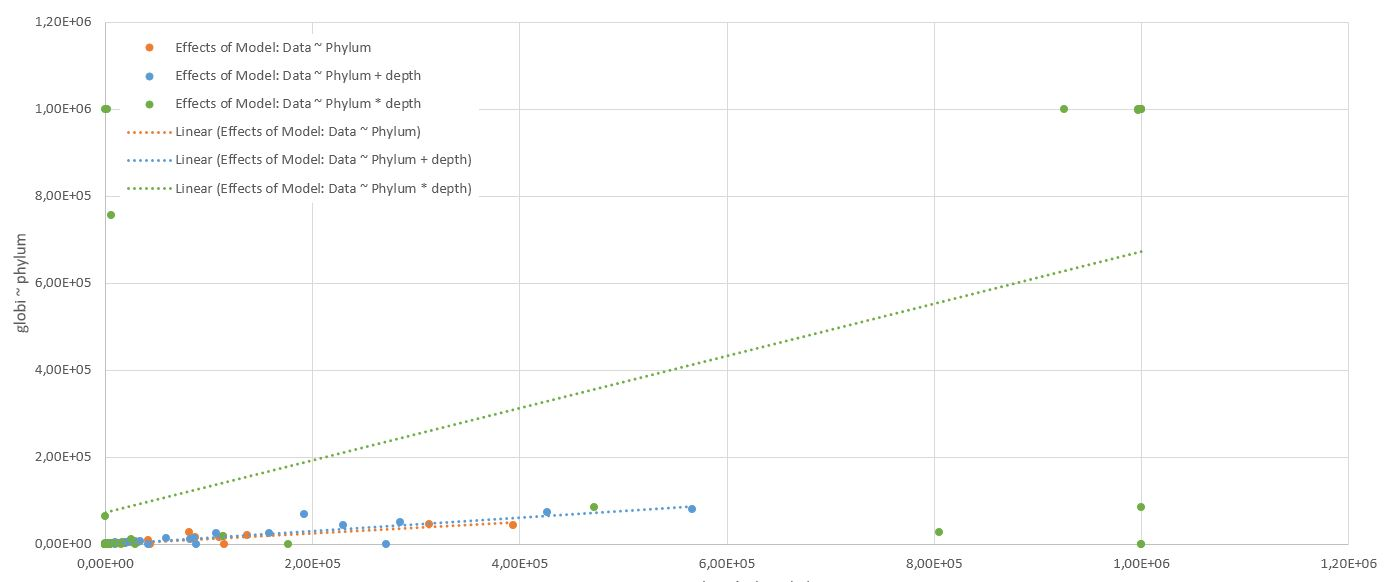
\includegraphics[trim = 0mm 0mm 0mm 0mm, clip, width=\textwidth]{Figures/EffectsOf3Models-Data-Phylum.JPG}
      \caption{Effects of 3 Models: Data $\sim$ Phylum (+/* depth)}
      \label{fig:...}
    \end{figure}
    \begin{figure}[h!]
      \centering
      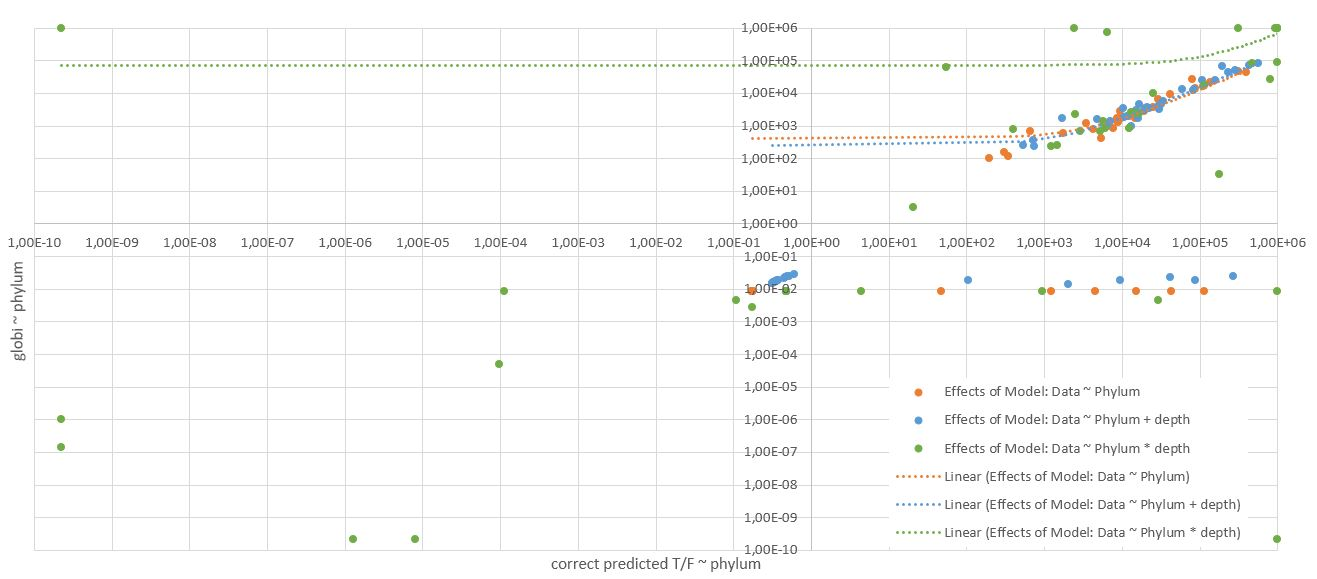
\includegraphics[trim = 0mm 0mm 0mm 0mm, clip, width=\textwidth]{Figures/EffectsOf3Models-Data-Phylum_loglog.JPG}
      \caption{Effects of 3 Models: Data $\sim$ Phylum (+/* depth) \\ both axis in log scale}
      \label{fig:...}
    \end{figure}

%---------------------------------------------------------------------------------------------------
%---------------------------------------------------------------------------------------------------
%---------------------------------------------------------------------------------------------------
%---------------------------------------------------------------------------------------------------
\chapter{Discussion}

  Fehlerqoute der Daten an sich? \\
  Wie gut ist unsere Datenlage? 3 mio knoten, 1.8 named species (leaf nodes), 200.000 leaf nodes mit 
  Information. \\
  Welche Teile des Baumes sind gut, an welchen muss noch viel geforscht werden. \\
  Wieviele Origins haben wir gefunden, was bedeutet diese Zahl? \\
  Es gibt noch ungenutze information in GloBI.

  %---------------------------------------------------------------------------------------------------
  %---------------------------------------------------------------------------------------------------
  %---------------------------------------------------------------------------------------------------
  \section{Simulation}
    For fixed calculations we assume a distribution of 60\% free-living to 40\% parasites, 95\% 
      missing data and a multifuration rate of 95\%.
    How well does our simulation approach the real data situation? \\
    There are some points to discuss:
    \begin{itemize}
      \item How close is the randomized binary tree to a true phylogeny?
      \item The distribution of parasites to free-ranging species is a pure assumption. From different 
        sources about 40\% parasites are estimated, are these also beta-distributed?
      \item How well do the transition probabilities match parasitism? Depending on the type of 
        parasitism, this will certainly look different. In addition, it can be assumed that the 
        probability for losses is lower than for origins.
      \item The equal distribution of the multifurcation is a blank assumption. It is very likely to 
        be higher towards the root node because there is less information back in time. On the other 
        hand, there are many studies that have studied various species without considering phylogeny. 
        Which also creates a high number of children of a node directly at the leaf nodes.
    \end{itemize}
    In order to be able to observe these problems, we have programmed our simulation according to the 
      parameters. This allowed us to estimate the influence of some of these parameters.

  
%---------------------------------------------------------------------------------------------------
%---------------------------------------------------------------------------------------------------
%---------------------------------------------------------------------------------------------------
\bibliography{bibliographie}

%---------------------------------------------------------------------------------------------------
%---------------------------------------------------------------------------------------------------
%---------------------------------------------------------------------------------------------------
\chapter{Appendices}
  %---------------------------------------------------------------------------------------------------
  %---------------------------------------------------------------------------------------------------
  \section{OTL analysis}\label{sec:otl analysis}

    %---------------------------------------------------------------------------------------------------
    \subsection{List of all phyla}\label{subsec:listPhyla}

    Phyla (53): \\
    Acanthocephala, Amoebozoa, Apicomplexa, Arthropoda, Ascomycota, Bacillariophyta, Basidiomycota, 
      Brachiopoda, Bryozoa, Chaetognatha, Chlorophyta, Chordata, Chromerida, Chytridiomycota, 
      Ciliophora, Cnidaria, Colponemidia, Ctenophora, Cycliophora, Echinodermata, Entoprocta, 
      Entorrhizomycota, Euglenida, Foraminifera, Gastrotricha, Glomeromycota, Gnathostomulida, 
      Haplosporida, Haptophyta, Hemichordata, Kinorhyncha, Loricifera, Microsporidia, Mollusca, 
      Myzostomida, Nematoda, Nematomorpha, Nemertea, Onychophora, Orthonectida, Phaeophyceae, 
      Picozoa, Placozoa, Platyhelminthes, Porifera, Priapulida, Rhodophyta, Rhombozoa, Rotifera, 
      Streptophyta, Tardigrada, Xanthophyceae \\
    Wobei von Streptophyta -> Anthocerotophyta, Marchantiophyta, Bryophyta, Tracheophyta als
      Phylum im Phylum gefunden und nicht einbezogen wurden und Magnoliophyta als Phylum in 
      Tracheophyta ebenfalls nicht. \\

    %---------------------------------------------------------------------------------------------------
    \subsubsection{Distribution of Taxa}
    - In the tree we can distinguish 28 different Taxa with the OTL taxonomic tree. \\
    - The most of them are hardly represented. The major taxonomic groups are: ... \\
    - Here you can see some characteristics of the Multifurcation of the tree. \\
    \begin{figure}[h!]
      \centering
      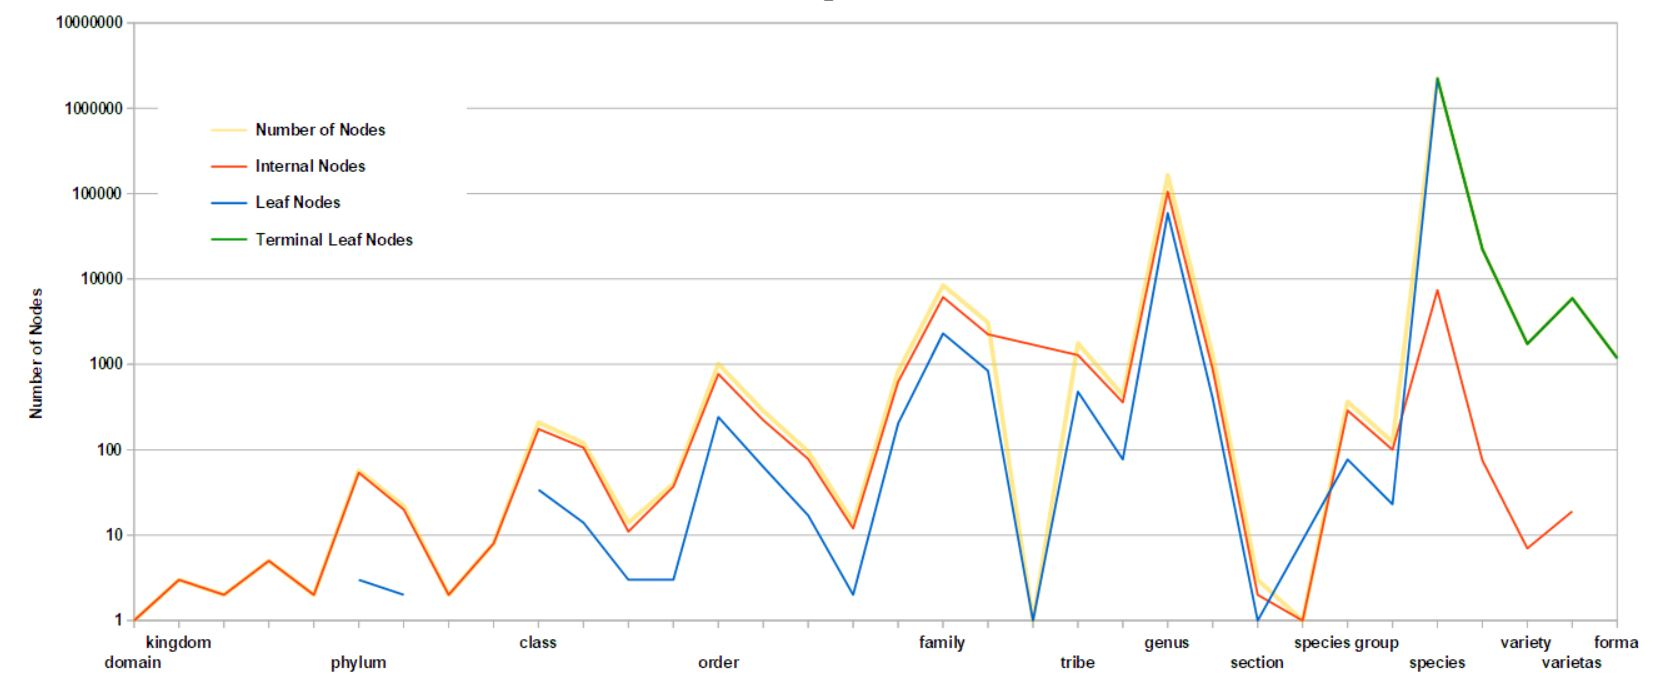
\includegraphics[width=0.9\textwidth]{Figures/TaxaTable2.JPG}
      \caption{Distribution of Nodes in Rank-Cathegories}
      \label{fig:taxaTable2}
    \end{figure}
    In a phylogeny, the taxonomic division of the tree is far too coarse, meaning that there should 
      be more subtaxa or 'unranked' nodes. But the closer we get to the root, the more the pure
      taxonomic tree is reflected. If the tree were binary, the taxa would have to double. But the 
      multipliers for some are much bigger and for others much smaller, which you can see in in figure 
      \ref{fig:taxaTable2}. \\
      ... (see Table \ref{table:...})
    
    \begin{table}[h!]
      \begin{center}
        % \begin{tabular}{ |>{\rowmac}l|>{\rowmac}r|<{\clearrow} }
        \begin{tabular}{ |l|r||r|r|r| }
          \hline
          Taxa & Number of Nodes & Internal Nodes & Leaf Nodes & Terminal Leaf Nodes \\
          \hline \hline
          \setrow{\bfseries}domain & 1 & 1 & &  \\ \hline
          \setrow{\bfseries}kingdom & 3 & 3 & &  \\
          subkingdom & 2 & 2 & & \\
          infrakingdom & 5 & 5 & & \\
          superphylum & 2 & 2 & & \\ \hline
          \setrow{\bfseries}phylum & 57 & 54 & 3 & \\
          subphylum & 22 & 20 & 2 & \\
          infraphylum & 2 & 2 & & \\
          superclass & 8 & 8 & & \\ \hline
          \setrow{\bfseries}class & 209 & 175 & 34 & \\
          subclass & 120 & 106 & 14 & \\
          infraclass & 14 & 11 & 3 & \\
          superorder & 40 & 37 & 3 & \\ \hline
          \setrow{\bfseries}order & 1014 & 772 & 242 & \\
          suborder & 285 & 222 & 63 & \\
          infraorder & 95 & 78 & 17 & \\
          parvorder & 14 & 12 & 2 & \\
          superfamily & 829 & 626 & 203 & \\ \hline
          \setrow{\bfseries}family & 8449 & 6143 & 2306 & \\
          subfamily & 3090 & 2250 & 840 & \\
          supertribe & 1 & 0 & 1 & \\
          tribe & 1764 & 1285 & 479 & \\
          subtribe & 435 & 359 & 77 & \\ \hline
          \setrow{\bfseries}genus & 164656 & 105452 & 59204 & \\
          subgenus & 1266 & 869 & 397 & \\
          section & 3 & 2 & 1 & \\
          subsection & 1 & 1 & 0 & \\
          species group & 365 & 288 & 77 & \\
          species subgroup & 123 & 100 & 23 & \\ \hline
          \setrow{\bfseries}species & 2247251 & 7423 & 2239828 & 2228993 \\
          subspecies & 22437 & 75 & 22362 & 22239 \\
          variety & 1755 & 7 & 1748 & 1726 \\
          varietas & 5970 & 19 & 5951 & 5909 \\
          forma & 1181 & & 1181 & 1181 \\
          \hline \hline
          no rank & 954 & 719 & 235 & 7 \\
          no rank - terminal & 37452 & & 37452 & 37452 \\
          (no entry) & 40099 & 40099 & & \\
          \hline  
        \end{tabular}
        \caption{\todo{...}}
        \label{table:...} 
      \end{center}  
    \end{table}
    extended leaf nodes (real leaf nodes)

  %---------------------------------------------------------------------------------------------------
  \subsubsection{Distribution of data in the taxa}
    Mithilfe des taxonomischen Baums von OTL haben wir die Knoten ihren Kingdoms, Phyla und Classes 
      zugeteilt (see Table \ref{table:...}). \\

    \begin{table}[h]
      \begin{center}
        \begin{tabular}{ |l|r|l|r|r| }
          \hline
          Kingdom (3) & Number of Nodes & Phylum (25) & Number of Nodes & max max height \\
          \hline \hline
          Metazoa & 1 465 207 & Arthropoda & 1 170 539 & 54 \\
          & & Chordata & 106 650 & 74 \\
          & & Mollusca & 80 022 & 22 \\
          & & Platyhelminthes & 27 141 & 9 \\
          & & Nematoda & 24 564 & 23 \\
          & & Cnidaria & 14 878 & 36 \\
          & & Porifera & 11 737 & 26 \\
          & & Echinodermata & 10 654 & 14 \\
          & & Bryozoa & 8 631 & 11 \\
          & & Rotifera & 3 093 & 7 \\
          & & Nemertea & 1 793 & 7 \\
          & & Tardigrada & 1 654 & 7 \\
          & & Acanthocephala & 1 596 & 6 \\
          & & Brachiopoda & 1 055 & 9 \\
          & & Nematomorpha & 633 & 7 \\
          & & Chaetognatha & 360 & 7 \\
          & & Hemichordata & 196 & 5 \\ 
          & & Cycliophora & 11 & 5 \\ 
          % 1465207-(1170539+106650+80022+27141+24564+14878+11737+10654+8631+3093+1793+1654+1596+1055+633+360+196+11) = 0          \hline
          Fungi & 254 871 & Ascomycota & 157 045 & 19 \\ 
          & & Basidiomycota & 92 931 & 18 \\
          & & Microsporidia & 1 949 & 6 \\ 
          & & Glomeromycota & 1 490 & 6 \\
          & & Chytridiomycota & 1 456 & 6 \\
          % 254871-157045-92931-1949-1490-1456 = 0
          \hline
          Chloroplastida & 121 239 & Streptophyta & 120 731 & 49 \\
          & & Chlorophyta & 508 & 6 \\
          % 121239-120731-508 = 0
          \hline  
        \end{tabular}
        \caption{\todo{...}}
        \label{table:...} 
      \end{center}  
    \end{table}

\end{document}